%%%%%%%%%%%%%%%%%%%%%%%%%%%%%%%%%%%%%%%%%%%%
% DMECS Dissertation
% LaTeX Template
% Version 0.5 (Jan 2026)
%
% Adapted to MESCC/ISEP by
% Luis Miguel Pinho (lmp@isep.ipp.pt) and
% António Barros (amb@isep.ipp.pt)
%
% Based on TMDEI/ISEP style (Dec/2015) by
%  Nuno Pereira (nap@isep.ipp.pt) and
%  Paulo Baltarejo (pbs@isep.ipp.pt)
%
% Based on MastersDoctoralThesis Version 1.2 by Vel (vel@latextemplates.com) and
% Johannes Böttcher, downloaded from (21/11/15):
% http://www.LaTeXTemplates.com
%
% This template is originally based on a template by:
% Steve Gunn (http://users.ecs.soton.ac.uk/srg/softwaretools/document/templates/)
% Sunil Patel (http://www.sunilpatel.co.uk/thesis-template/)
%
% Template license:
% CC BY-NC-SA 3.0 (http://creativecommons.org/licenses/by-nc-sa/3.0/)
%
%%%%%%%%%%%%%%%%%%%%%%%%%%%%%%%%%%%%%%%%%

%----------------------------------------------------------------------------------------
%	PACKAGES AND OTHER DOCUMENT CONFIGURATIONS
%----------------------------------------------------------------------------------------

\documentclass[
	11pt, % The default document font size, options: 10pt, 11pt, 12pt
	%oneside, % Two side (alternating margins) for binding by default, uncomment to switch to one side (for drafting/reading purposes)
	english, % english for English;
	%portuguese, % for Portuguese; delete temporary files if you change language (e.g. 'make clean; make')
	%singlespacing, % Single line spacing, alternatives: onehalfspacing or doublespacing (for drafting/reading purposes)
	onehalfspacing, % AMB: Specified by the ISEP template guidelines.
	%draft, % Uncomment to enable draft mode (no pictures, no links, overfull hboxes indicated)
	nolistspacing, % If the document is onehalfspacing or doublespacing, uncomment this to set spacing in lists to single
	%liststotoc, % Uncomment to add the list of figures/tables/etc to the table of contents (not recommended)
	%toctotoc, % Uncomment to add the main table of contents to the table of contents (not recommended)
	parskip, % Add space between paragraphs (recommended)
	%nohyperref, % Uncomment to not load the hyperref package (not recommended)
	nohyperreflinkcolor, % hyperref links are not colored (comment to color links, for example to produce an electronic-only version)
	headsepline, % Uncomment to get a line under the header
]{dmesc-style} % The class file specifying the document structure

\usepackage{tikz} % Required for creating graphics programmatically (can be removed if not used)
%\usetikzlibrary{arrows} % Required for fancy arrows in TiKZ graphics (can be removed if not used)

\usepackage{pgfplots} % Required for drawing high--quality function plots (can be removed if not used)
\pgfplotsset{compat=newest}

%
% Next you have examples of admissable citation styles; we recomend using the authoryear-comp citation style (which resembles Harvard); don't forget to only uncomment one
%

% authoryear-comp: recommended citation style (e.g. (Buendía, 1860), (Buendía 1910, Arcadio 1940))
% AMB: USE THIS STYLE, according to ISEP dissertation guidelines.
\usepackage[style=authoryear-comp,backend=biber]{biblatex} % Bibtex backend with the authoryear-comp citation style (authoryear citations, bibliography ordered alphabetically)

% numeric citation style (e.g. [1], [1-3])
% AMB: DO NOT USE THIS STYLE, according to ISEP dissertation guidelines.
%\usepackage[style=numeric-comp,sorting=none,backend=biber]{biblatex} % Bibtex backend with the numeric-comp citation style (numeric citations, bibliography ordered by appearance)

% alphabetic citation style (e.g. [Buendía10], [Buendía10, Arcadio40])
% AMB: DO NOT USE THIS STYLE, according to ISEP dissertation guidelines.
%\usepackage[style=alphabetic,sorting=none,backend=biber]{biblatex} % Bibtex backend with the alphabetic citation style (alphabetic citations, bibliography ordered by appearance)

\usepackage{url}

\usepackage{tabularx}

\usepackage{listings}

\lstdefinestyle{rustblock}{
    language=Rust,
    basicstyle=\ttfamily\small,
    frame=none,
    columns=fullflexible,
    keepspaces=true,
    showstringspaces=false,
    breaklines=true
}

\lstdefinestyle{cppblock}{
    language=C++,
    basicstyle=\ttfamily\small,
    numbers=left,
    numberstyle=\tiny,
    frame=single,
    breaklines=true,
    breakatwhitespace=false,
    columns=fullflexible
}

\addbibresource{mainbibliography.bib} % The filename of the bibliography

\makeglossaries % build the glossary


%----------------------------------------------------------------------------------------
%	THESIS INFORMATION
%----------------------------------------------------------------------------------------

\thesistitle{Modernizing C++ Legacy Systems with Rust: Strategies for Safe Interoperability and Performance Evaluation in Rust-Based Boost Components} % Your thesis title, this is used in the title, print it elsewhere with \ttitle

%\thesissubtitle{Subtitle (if exists)} % Your thesis subtitle, this is used in the title, print it elsewhere with \tsubtitle, comment line if not existing

\author{Filipe Daniel Ferreira} % Your name, this is used in the title page, print it elsewhere with \authorname

\supervisor{Luis Miguel Pinho} % Your supervisor's name, this is used in the title page, print it elsewhere with \supname

%\cosupervisor{Full Name (if exists)} % Your co-supervisor's name, this is used in the title page, print it elsewhere with \cosupname (comment, if no co-supervisor)

%\externalsupervisor{Full Name (if exists)} % Your external (company) supervisor's name, this is used in the title page, print it elsewhere with \extsupname (comment, if no external supervisor)

%\committeepresident{Full Name, Category, Affiliation} % Name of the president of the evaluation committee, print it elsewhere with \presidentname


% \committeemembers{}

%\committeemembers{Full Name, Category, Affiliation\\Full Name, Category, Affiliation} % Name of the evaluation committee members (up to four), print it elsewhere with \committee

\keywords{Boost, C++, Rust, interoperability, migration, memory safety} % Please define up to 6 keywords that better describe your work, print it elsewhere with \keywordnames

\thesisdate{Porto, \today} % thesis date,  print it elsewhere with \tdate

\hypersetup{pdftitle=\ttitle} % Set the PDF's title to your title
\hypersetup{pdfauthor=\authorname} % Set the PDF's author to your name
\hypersetup{pdfkeywords=\keywordnames} % Set the PDF's keywords to your keywords

%----------------------------------------------------------------------------------------
%	THE CONTENT OF THE DOCUMENT BEGINS HERE
%----------------------------------------------------------------------------------------

\begin{document}


%----------------------------------------------------------------------------------------
%	FRONT MATTER
%----------------------------------------------------------------------------------------

% Include the frontmatter of your thesis here

% we include the glossary here (frontmatter is included with \input, so this command is as if it was in main.tex)
%All acronyms must be written in this file.
\newacronym{SDV}{SDV}{Software Defined Vehicles}
\newacronym{FFI}{FFI}{Foreign Function Interfaces}
\newacronym{ECU}{ECU}{Electronic Control Units}
\newacronym{RTS}{RTS}{Real-Time System}
\newacronym{GPOS}{GPOS}{General Purpose Operating System}
\newacronym{RTOS}{RTOS}{Real-Time Operating System}
\newacronym{PGF}{PGF}{Portable Graphics Format}
\newacronym{RAII}{RAII}{Resource Acquisition Is Initialization}
\newacronym{STD}{STD}{Standard C++ library}
\newacronym{TMP}{TMP}{Template Metaprogramming}
\newacronym{CWE}{CWE}{Common Weakness Enumeration}
\newacronym{SCORE}{SCORE}{Safety-Critical Open Research Environment}
\newacronym{ASIL}{ASIL}{Automotive Safety Integrity Levels}
\newacronym{QM}{QM}{Quality Management}
\newacronym{WCET}{WCET}{Worst Case Execution Time}


\newacronym{X}{X}{X}

\frontmatter % Use roman page numbering style (i, ii, iii, iv...) for the pre-content pages

\pagestyle{plain} % Default to the plain heading style until the thesis style is called for the body content

%----------------------------------------------------------------------------------------
%	TITLE PAGE
%----------------------------------------------------------------------------------------

\maketitlepage


%----------------------------------------------------------------------------------------
%	STATEMENT of INTEGRITY
%----------------------------------------------------------------------------------------

\integritystatement


%----------------------------------------------------------------------------------------
%	DEDICATION  (optional)
%----------------------------------------------------------------------------------------
%
%\dedicatory{For/Dedicated to/To my\ldots}
% \begin{dedicatory}

%The dedicatory is optional. 

% \end{dedicatory}


%----------------------------------------------------------------------------------------
%	ABSTRACT PAGE
%----------------------------------------------------------------------------------------

\begin{abstract}

The growing complexity of safety-critical software systems, particularly in the automotive domain, 
has intensified concerns regarding memory safety, concurrency correctness 
and long-term maintainability of large C++ codebases. Although C++ remains the dominant language in embedded and 
real-time systems due to its performance and mature ecosystem, 
its reliance on manual memory management continues to be a major source of vulnerabilities. 
Rust has emerged as a promising alternative, offering strong compile-time guarantees for memory safety 
and data-race freedom without introducing garbage collection. 
However, the adoption of Rust in industrial environments is hindered by the scale of existing C++ systems 
and their deep dependence on template-heavy frameworks such as the Boost C++ Libraries.

This dissertation investigates strategies for incrementally modernizing legacy C++ systems by integrating Rust in a safe 
and performant manner. Focusing on Boost-based components commonly used in automotive software architectures, 
it proposes a systematic methodology for selecting migration candidates, designing bidirectional interoperability interfaces, 
and re-implementing critical functionality in Rust. The work explores \gls{FFI} patterns, 
evaluates existing interoperability tools, and addresses the architectural challenges arising from the mismatch 
between C++ templates and Rust’s ownership model.

A Rust-based reimplementation of selected Boost components is developed and integrated into a hybrid C++/Rust system. 
Performance, memory usage, and interoperability overhead are experimentally evaluated to quantify the benefits 
and costs of this approach. The results demonstrate that incremental migration can significantly improve memory safety 
while preserving determinism and performance, providing practical guidance for the adoption of Rust in high-assurance 
and safety-critical software systems.

\end{abstract}

\begin{abstractotherlanguage}
A crescente complexidade dos sistemas de software crítico e seguro, particularmente no domínio automóvel, 
intensificou as preocupações relativas à segurança da memória, à correção da concorrência 
e à manutenção a longo prazo de grandes bases de código C++. Embora o C++ continue a ser a linguagem dominante 
em sistemas embebidos e de tempo real devido ao seu desempenho e ecossistema maduro, 
a sua dependência da gestão manual da memória continua a ser uma importante fonte de vulnerabilidades. 
O Rust surgiu como uma alternativa promissora, oferecendo fortes garantias em tempo de compilação para a segurança da memória 
e a ausência de conflitos de dados, sem introduzir a recolha de lixo. 
No entanto, a adoção do Rust em ambientes industriais é dificultada pela escala dos sistemas C++ existentes 
e sua profunda dependência de frameworks fortemente baseadas em modelos, como as bibliotecas Boost C++.

Esta dissertação investiga estratégias para modernizar incrementalmente sistemas C++ antigos, integrando Rust de maneira segura 
e com bom desempenho. Com foco em componentes baseados em Boost comumente usados em arquiteturas de software automotivo, 
ela propõe uma metodologia sistemática para selecionar candidatos à migração, projetar interfaces de interoperabilidade 
bidirecionais e reimplementar funcionalidades críticas em Rust. O trabalho explora padrões de \gls{FFI}, 
avalia ferramentas de interoperabilidade existentes e aborda os desafios arquitetônicos decorrentes da incompatibilidade 
entre modelos C++ e o modelo de propriedade do Rust.

Uma reimplementação baseada em Rust de componentes Boost selecionados é desenvolvida e integrada a um sistema híbrido C++/Rust. 
O desempenho, o uso de memória e a sobrecarga de interoperabilidade são avaliados experimentalmente para quantificar os benefícios 
e custos dessa abordagem. Os resultados demonstram que a migração incremental pode melhorar significativamente a segurança da memória ,
preservando o determinismo e o desempenho, fornecendo orientações práticas para a adoção do Rust em sistemas de software de alta garantia 
e segurança crítica.

\end{abstractotherlanguage}


%----------------------------------------------------------------------------------------
%	ACKNOWLEDGEMENTS (optional)
%----------------------------------------------------------------------------------------

% \begin{acknowledgements}

%Acknowledgements (optional) to family, supervisors, colleagues, organizations, funding agencies, …

% \end{acknowledgements}


%----------------------------------------------------------------------------------------
%	LIST OF CONTENTS/FIGURES/TABLES PAGES
%----------------------------------------------------------------------------------------

\tableofcontents % Prints the main table of contents

\listoffigures % Prints the list of figures

\listoftables % Prints the list of tables

%\iflanguage{portuguese}{
%\renewcommand{\listalgorithmname}{Lista de Algor\'itmos}
%}
%\listofalgorithms % Prints the list of algorithms
%\addchaptertocentry{\listalgorithmname}


%\renewcommand{\lstlistlistingname}{List of Source Code}
%\iflanguage{portuguese}{
%\renewcommand{\lstlistlistingname}{Lista de C\'odigo}
%}
%\lstlistoflistings % Prints the list of listings (programming language source code)
%\addchaptertocentry{\lstlistlistingname}


%----------------------------------------------------------------------------------------
%	ABBREVIATIONS
%----------------------------------------------------------------------------------------
\begin{abbreviations}{ll} % Include a list of abbreviations (a table of two columns)
%\textbf{LAH} & \textbf{L}ist \textbf{A}bbreviations \textbf{H}ere\\
%\textbf{WSF} & \textbf{W}hat (it) \textbf{S}tands \textbf{F}or\\
\end{abbreviations}

%----------------------------------------------------------------------------------------
%	SYMBOLS
%----------------------------------------------------------------------------------------

%\begin{symbols}{lll} % Include a list of Symbols (a three column table)

% [Note: Although acronyms and symbols are defined in this section, they should also be defined at least the first time used in the dissertation body.]

%$a$ & distance & \si{\meter} \\
%$P$ & power & \si{\watt} (\si{\joule\per\second}) \\
%Symbol & Name & Unit \\

%\addlinespace % Gap to separate the Roman symbols from the Greek

%$\omega$ & angular frequency & \si{\radian} \\

%\end{symbols}



%----------------------------------------------------------------------------------------
%	ACRONYMS
%----------------------------------------------------------------------------------------

\newcommand{\listacronymname}{List of Acronyms}
\iflanguage{portuguese}{
\renewcommand{\listacronymname}{Lista de Acr\'onimos}
}

%Use GLS
\glsresetall
\printglossary[title=\listacronymname,type=\acronymtype,style=long]

%----------------------------------------------------------------------------------------
%	DONE
%----------------------------------------------------------------------------------------

\mainmatter % Begin numeric (1,2,3...) page numbering
\pagestyle{thesis} % Return the page headers back to the "thesis" style


%----------------------------------------------------------------------------------------
%	MAIN BODY
%----------------------------------------------------------------------------------------

% Include the chapters of the thesis as separate folder for each chapter
% Uncomment the lines as you write the chapters

% Chapter 1
% 
\chapter{Introduction} % Main chapter title
\label{chap:Chapter1} % For referencing the chapter elsewhere, use Chapter~\ref{chap:Chapter1}


%-------------------------------------------------------------------------------
%---------
%
\section{High-Level Overview and Motivation} 
\label{sec:high_level_overview} 
The automotive industry is performing a profound transformation driven by the rise of the \gls{SDV}, 
autonomous driving technologies and increasingly interconnected \gls{ECU} \parencite{spglobalsdv}. 
With the grouth of these systems in complexity and responsability, the reliability of high-assurance software becomes critical. 
The systems must operate under strict real-time, reliability and safety requeriments regulated by standards as ISO 26262 \parencite{deloittesdvreadiness}. 
In this environment, memory safety has a special importance, as software faults can directly translate into physical hazards \parencite{adacore_nsa_cisa_msl}.

Historically, C++ has been the dominant language (paired with C) in embedded and automotive development due to its performance, 
deterministic resource use and mature ecosystem \parencite{ISO26262_Part6}. 
However, its dependence on manual memory management continues to be a major source of vulnerabilities such as: 
buffer overflows, dangling pointes, race conditions and undefined behaviors \parencite{MISRACpp2023}. 
Such issues are incompatible with the needs ofsafety critical cyber-physical systems, 
where a minor software defect can lead to serious consequences \parencite{AUTOSAR_Adaptive}.

Rust has rapidly emerged as a plausible successor for safety-critical software. 
Enforcing memory safety, ownerhip and data race free concurrency at compile time \parencite{docs_rs}. 
Rust promises to drastically reduce classes of defects edemic to C/C++ systems \parencite{ProgrammingRust}. 
Rust achieves this without introducing garbage collection, which can support predictable resource management in systems with real-time requirements \parencite{docs_rs}.

Despite the advantages Rust presents, the transition from C++ to Rust in large industrial ecosystems remains complex. 
Automotive software contains millions of lines of validated legacy C++ code. 
This code is oftenly built at top of complex frameworks and libraries as Boost C++ libraries \parencite{CXX_Crate}. 
Rewrinting those systems from scratch is infeasible. To avoid it, the companies usally pursue incremental and hybrid migration. 
This migration requires robust interoperability between Rust and C++ \parencite{Google_Rust_Interop}.

This dissertation is motivated byt the need to address that gap: 
enabling safe, practical and measurable integration of Rust into deeply entrenched C++ based automotive architectures, 
specially real-time related architectures.

Rewriting millions of lines of validated, legacy C++ code is operationally infeasible, 
necessitating a hybrid integration strategy. 
This transition is particularly problematic for automotive subsystems (such as sensor fusion, V2X communication and path planning) 
that are deeply coupled with the C++ ecosystem and reliant on complex, template-heavy frameworks like the Boost C++ Libraries.


\section{Problem Statement} 
\label{sec:problem_statement} %For referencing this section elsewhere, use Section~\ref{sec:problem_statement}

The central results from the tension between two different realities:
\begin{enumerate}
    \item \textbf{C++ is deeply entrenched in automotive systems}, specially through heavily templated, performance-critical frameworks like Boost.
    \item  \textbf{Rust provides strong memory safety guarantees}, but its adoption is hindered by the difficulty of interoperating with complex C++ abstrations creating a challenge for a transition between C++ and Rust. 
\end{enumerate} 

Currently, the interoperability approaches rely mainly on C-style \gls{FFI} . 
However, ist not possiblet to natively represent C++ templates, ownership semantics, 
RAII lifecycles or advanced Boost abstractions with C \gls{FFI} \parencite{CrubitDesign}.

As result of this limitation:
\begin{itemize}
    \item The integration often requires unsafe code, reducing Rust's safety benefits.
    \item Interfacing with templaty heavily libraries, as Boost.Geometry and Boost.Asio, introduces high engineering overhead.
    \item Crossing the Rust and C++ boundary imposes a performance cost that is poorly characterized for high-assurance systems.
    \item The reviewed literature does not provide a sufficiently detailed methodology for the systematic and incremental migration of C++ Boost components to Rust while maintaining compatibility with automotive subsystems.
\end{itemize}

The problem is not simply porting code from C++ to Rust, but the absence of validated techniques, architectural patterns, and tooling to bridge the impedance mismatch between C++ templates and Rust's ownership model, without breaking determinism, performance or safety requirements.


\section{Research Questions}
\label{sec:research_questions}

To address the research gap, this dissertation is guided by the following research questions:
\begin{enumerate}
    \item \textbf{RQ1:} What architectural and interoperability patterns can support the incremental migration of selected Boost components from C++ to Rust?
    \item \textbf{RQ2:} What criteria can be used to identify Boost components that are suitable candidates for incremental migration in automotive-oriented software?
    \item \textbf{RQ3:} How can selected Boost components be reimplemented using Rust abstractions while preserving their relevant observable behaviour?
    \item \textbf{RQ4:} How can Rust/C++ FFI boundaries be designed to explicitly manage ownership, representation, lifetime, and error-handling constraints?
    \item \textbf{RQ5:} What performance characteristics are observed when the selected Rust implementations are compared with their C++ counterparts under the evaluated workloads?
    \item \textbf{RQ6:} Which safety guarantees are provided by Rust within the migrated components, and which guarantees must remain explicit contracts at the FFI boundary?
\end{enumerate}

The questions are intentionally scoped to the selected case studies and evaluated workloads. In particular, the performance experiments measure observed execution time and throughput rather than worst-case execution time, and therefore do not establish hard real-time guarantees.

\section{Research Objectives}
\label{sec:research_objectives}

The primary objective of this dissertation is to design, implement and evaluate a methodology for the incremental migration of selected Boost C++ components into Rust, while maintaining controlled interoperability with existing C++ systems. The work focuses on identifying repeatable migration decisions, applying them to two representative low-level libraries, and evaluating the resulting technical trade-offs.

The specific objectives are:
\begin{itemize}
    \item Analyze existing interoperability mechanisms between Rust and C++, including C ABI based integration, \texttt{cxx}, \texttt{bindgen}, \texttt{autocxx}, and \texttt{cbindgen}.
    \item Define explicit criteria for selecting Boost components suitable for migration, including safety relevance, isolation, portability, interoperability, performance relevance, and implementation complexity.
    \item Select and reimplement representative functionality from \texttt{Boost.Align} and \texttt{Boost.Endian} using Rust-native abstractions rather than performing a purely syntactic translation.
    \item Design interoperability boundaries with explicit ownership, lifetime, representation, and error-handling contracts.
    \item Measure functional correctness, selected performance characteristics, memory behaviour, and FFI overhead for the implemented case studies.
    \item Identify migration patterns that are generalizable beyond the two selected libraries and distinguish them from decisions that are specific to their APIs or compatibility requirements.
    \item Characterize the limitations of the evaluated approach, particularly at unsafe Rust and Rust/C++ FFI boundaries.
\end{itemize}

\section{Research Contributions}
\label{sec:research_contributions}

The contributions of this dissertation are:
\begin{itemize}
    \item A structured set of criteria for assessing Boost components as incremental Rust migration candidates.
    \item A comparative analysis of Rust/C++ interoperability mechanisms with explicit attention to compatibility, safety, portability, performance, ABI stability, and build complexity.
    \item A migration methodology that emphasizes semantic analysis, Rust-native redesign, explicit interoperability contracts, validation, and critical analysis of residual risks.
    \item Rust-native reimplementations of selected functionality from \texttt{Boost.Align} and \texttt{Boost.Endian}, demonstrating two different FFI strategies.
    \item An analysis of unsafe-code and FFI boundaries, including the safety properties that remain enforceable inside Rust and those that become external contracts.
    \item A quantitative evaluation of the selected implementations, including execution time, throughput, memory observations, correctness checks, and FFI overhead.
\end{itemize}

\section{Dissertation Plan Structure}
\label{sec:dissertation_structure}

The remainder of this dissertation is organized as follows:
\begin{itemize}
    \item \textbf{Chapter 2 -- State of the Art:} Presents the technological background, related work, Rust/C++ interoperability mechanisms, Boost architecture, and the criteria used to compare interoperability approaches.
    \item \textbf{Chapter 3 -- Methodology and Solution Proposal:} Defines the component-selection criteria, migration-enabling rationale, and proposed architectural methodology.
    \item \textbf{Chapter 4 -- Migration Strategy:} Describes the systematic migration process used to analyse, redesign, implement, integrate, and validate selected Boost functionality.
    \item \textbf{Chapter 5 -- Selected Libraries:} Describes \texttt{Boost.Align} and \texttt{Boost.Endian}, their relevance to the study, and their selection as representative low-level case studies.
    \item \textbf{Chapter 6 -- Implementation, Evaluation and Critical Analysis:} Presents the Rust implementations, benchmark results, unsafe-code analysis, FFI safety analysis, and generalizable migration patterns.
    \item \textbf{Chapter 7 -- Conclusions and Future Work:} Summarizes the findings, answers the research questions, states the contributions and limitations, and identifies future work.
\end{itemize}

\section{Privacy and ethics}
In the context of this dissertation plan, which is focused in modernizing C++ based systems using Rust, 
ethical considerations were primarily centered on scientific integrity, software safety and intellectual property compliance.

The research relied on public open-source codebases, as Boost libraries.  No personal data, user-identifiable information (PII), or private operational logs were collected, processed, or stored. 
Consequently, the study falls outside the scope of GDPR requirements regarding human subjects.


\section{Use of AI Tools}
\label{sec:ai_tools}

For the preparation of this dissertation plan and supporting documentation, 
AI tools (specifically large language models) were used strictly for the following purposes:
\begin{itemize}
    \item \textbf{Document writing evaluation and improvement}, including linguistic refinement, clarity enhancement, and reorganization of text originally written by the author.
    \item \textbf{Assistance in identifying potential sources and directions for literature review}, such as suggesting relevant topics, keywords, and areas of research to investigate. All cited references included in the dissertation were individually verified, read, and selected by the author.
    \item Structural feedback and general writing suggestions for non-technical sections.
    \item Code example generation to support the investigation of the state of the art and also to facilitate the understanding.
\end{itemize}

The tools used were Perplexity (latest version), for deep search specialy for community based information, 
chat GPT (version GPT\-5.1) and Gemini (version 3), for document writing evaluation and improvement.

No AI-generated technical explanations, conceptual developments, design decisions, code, 
or analysis results were incorporated directly into the dissertation. 
All technical content is exclusively authored by the candidate.

The author takes full responsibility for the correctness, originality, and academic integrity of the work presented. If additional AI tools are used during the subsequent stages of the dissertation, this section will be updated accordingly to specify which tools were used, for what purpose, and in which components of the document. If no further AI usage occurs, this will also be explicitly stated.

% Chapter 2

\chapter{State of the art} % Main chapter title

\label{chap:Chapter2} % For referencing the chapter elsewhere, use \ref{chap:Chapter2} 

%----------------------------------------------------------------------------------------

The integration of Rust into C++ environments, particularly Boost libraries, marks a significant evolution in software development. 
Rust's core strengths are memory safety and concurrency without garbage collection, 
addressing longstanding vulnerabilities in C++ systems. 
Recent studies on microcontroller applications show that Rust can have similar speed to C 
with lower energy use than interpreted languages. While performance evaluations on platforms, such as Raspberry Pi, 
indicates that Rust FFT implementations can match or exceed C in energy efficiency \parencite{dashdamirli2025analyzing,rooney2023evaluating}.

These characteristics are dominant in systems with strict deterministic requirements, 
such as automotive Electronic Control Units (ECUs), high-frequency trading platforms, and real-time robotics. 
In these domains, the non-determinism introduced by garbage-collection "stop-the-world" pauses is not appropriate due to 
hard real-time latency constraints. Furthermore, resource-constrained embedded environments often cannot afford 
the runtime overhead associated with managed languages. Rust solves this problem through an ownership model and a 
strict borrow checker enforced at compile time. By tracking the lifetime and scope of every value during compilation, 
Rust guarantees memory safety and data-race freedom without requiring a runtime garbage collector. \parencite{okawa2024performance} 
This ensures that the resulting binary maintains the predictable performance and low resource footprint of C++, 
while eliminating entire classes of bugs such as null pointer de-referencing and use-after-free errors.

\section{Rust}

\subsection{Overview}

Rust is a systems programming language focused on three goals: safety, speed, and concurrency \parencite{RustProgrammingLanguage}.

It is designed to ensure memory safety and high performance without relying on a garbage collector, present in languages as
Python or Java.

To not rely on garbage collection and to avoid common memory issues found in languages like C and C++, 
such as null pointer dereferencing, double frees, and segmentation faults, 
Rust was designed to be memory safe while offering comparable performance \parencite{RustCppProgrammers}.

\subsubsection{Ownership and Memory Safety}
Rust distinguishes itself through a rigorous ownership model, 
which manages memory through a strict set of rules enforced at compile time by the "borrow checker", 
without a garbage collector. \parencite{ProgrammingRust}

The garbage collector, used by Python and Java, is an automatic memory management process that helps programs to run efficiently.
Rust does not use it for memory management, instead it determines exactly when memory should be freed based on variable scope. \parencite{ProgrammingRust}

Within a program run, every value has a single "owner" and when the owner goes out of scope the value is dropped. 
Ownership can be transferred (moved) but not implicitly copied for complex types, preventing double-free errors. \parencite{ProgrammingRust}

I also possible to "borrow" values through references. 
The compiler ensures that references are always valid and a mutable references cannot exist while other references exists, 
preventing data races. \parencite{RustCppProgrammers}

Scope and ownership code example:

\begin{lstlisting}[language=Rust]
    fn main() {
    // 1. SCOPE AND OWNERSHIP
    {
        let s1 = String::from("hello"); // s1 owns the string
        // s1 is valid here
    } // s1 goes out of scope here; memory is automatically freed (dropped)
    
    // 2. MOVE SEMANTICS (Transferring Ownership)
    let s2 = String::from("complex type");
    let s3 = s2; // Ownership moved from s2 to s3
    
    // println!("{}", s2); // Error! s2 is invalid. Prevents double-free errors.
    println!("s3 owns the data: {}", s3);

    // 3. BORROWING (References)
    let mut s4 = String::from("data");
    
    // Immutable borrow
    let r1 = &s4; 
    let r2 = &s4; // Multiple immutable references are allowed
    println!("Read only: {} and {}", r1, r2);
    // r1 and r2 scopes end here (last usage)

    // Mutable borrow
    let r3 = &mut s4; 
    r3.push_str(" race"); // Modify the borrowed value
    // let r4 = &s4; // Error! Cannot have immutable ref while mutable ref exists
                     // This rule prevents data races.
    
    println!("Modified data: {}", r3);
}
\end{lstlisting}

\subsubsection{Tooling and ecosystem}
An high quality tooling is a strong base of the Rust development environment. The integrated package manager \textbf{Cargo}, documentation generator \textbf{rustdoc} and built-in testing framework significantly enhance developer productivity. The Rust package registry, crates.io, is an important source of libraries for different applications.

Beside the growing usage of Rust, it still relies on interoperability with C/C++ ecosystem, specially for low-level applications (eg. hardware interactions, graphics, legacy protocols). Interfacing Rust with foreign code is possible using through the \gls{FFI}. Usualy, an \gls{FFI} is functional and efficient but often requires carefull design of abstractions, specially when crossing language boundaries with different memory management models.

\subsubsection{Adoption and Industrial Applications}
Rust has been adopted by several domains, as:

\begin{itemize}
    \item Web browsers and rendering engines, as mozilla firefox \parencite{mozilla_rust_docs}.
    \item Cloud infrastructures, as AWS firecracker \parencite{FirecrackerProject}.
    \item Operating systems and kernel modules, as in Linux kernel \parencite{LinuxKernelRust}.
    \item Blockchain clients and cryptographic systems \parencite{RustBlockchain2024}.
    \item High performance networking and embedded systems \parencite{RustEmbedded}.
\end{itemize}

\section{C++ and the Boost Library}

\subsection{C++}

C++ is currently the dominant programming language due to its extensive ecosystem. 
It has hardware specific libraries, mature compilers, profiling and debugging tools and frameworks for high-performance computing. 
Is also used for a large group of companies for many years \parencite{stroustrup2013cpp}. 
It leads to massive codebases, thousands of lines of code that make large rewrites infeasible \parencite{CppCon2020}.

Some common industries that usually use C++ are telecommunications, automotive, finance, aerospace, 
gaming, real-time control and large scale cloud systems \parencite{Stroustrup2020}.

The main challenges these systems have is their modernization. Modernizing them while ensuring the continuity, 
comaptibility and performance is not easy. Due to this, 
languages that interoperate with C++ instead of replacing it are preferred.

The main strenghts of C++ are:
\begin{itemize}
    \item High performance (specially comparing with C) \parencite{Stroustrup2020}.
    \item Deterministic resource management through \gls{RAII} \parencite{stroustrup2013cpp}.
    \item Support for control of hardware and memory \parencite{stroustrup2013cpp}.
    \item String abstraction mechanisms as templates, operator overloading and generic programming \parencite{stroustrup2013cpp}.
    \item Mature tools, compilers, profiling and debugging ecosystems \parencite{CppCon2020}.
\end{itemize}

The evolution of C++ ISO standard introduced modern features as smart pointers, concurrency primitives, 
modules and constant evaluation, for safety improvement and expressiveness \parencite{ISO_Cpp2020}.


\textbf{\textit{C++ memory model and safety limitations}}

Beside all the advantages, C++ has memory and safety limitations. 
C++ is designed to give developers complete control over memory and resources lifetime. 
It leads to the following unsafe behaviors:
\begin{itemize}
    \item Use after free and dangling pointers \parencite{msrc2020memory}.
    \item Double frees \parencite{msrc2020memory}.
    \item Buffer overflows and out of bound access \parencite{msrc2020memory}.
    \item Iterator invalidation \parencite{stroustrup2013cpp}.
    \item Data races \parencite{stroustrup2013cpp}.
    \item Uninitialized memory reads \parencite{msrc2020memory}.
    \item Reliance on undefined behaviors \parencite{stroustrup2013cpp}.
\end{itemize}

Industry data confirms that memory-unsafe languages (primarily C and C++) account for the majority of security vulnerabilities. 
Google reports that 70\% of Chrome vulnerabilities stem from memory safety bugs \parencite{google2022memory}, 
and Microsoft reports similar figures across Windows components \parencite{msrc2020memory}. 
Although modern C++ attempts to mitigate issues through smart pointers and safer API design, 
legacy code and raw pointer usage remain widespread \parencite{CppCon2020}.

\textbf{\textit{C++ concurrency and data races}}

C++ has a standardized model of memory since C++ 11. 
Through \gls{STD}, C++ provides access to threads (for multi processing and for parallel execution) 
and atomics that are a powerful mechanism for managing concurrent access to shared data in multithreaded applications.
Also provides mutexes, locks and condition variables for safety memory access for multiple processes concurrently.

With all those features C++ provides a possibility of an high performance for parallel programs, 
but the correctness of C++ remains difficult.
That is due C++ not being capable of statically prevent data races, 
C++ allows aliasing and mutation via multiple paths, exposes low level memory order operations 
and relies on the developer to ensure invariants \parencite{Stroustrup2020}.

At following example is possible to see two threads modifying the same resource, the global variable \textbf{\textit{counter}}.
The modification is concurrently leading to a undefined behavior.

\begin{lstlisting}[language=C++]
    #include <iostream>
    #include <thread>
    #include <vector>

    int counter = 0; // Shared resource

    void increment() {
        for (int i = 0; i < 1000000; ++i) {
            // Data race occurs here: read-modify-write is NOT atomic
            counter++; 
        }
    }

    int main() {
        std::thread t1(increment);
        std::thread t2(increment);

        t1.join();
        t2.join();

        std::cout << "Final counter: " << counter << std::endl;
        // Expected: 2000000
        // Actual: Likely < 2000000 (e.g., 146377) due to race conditions [web:51]
        return 0;
}
\end{lstlisting}

The incremental of \textbf{\textit{counter}}, \textbf{counter++}, is not atomic. 
Usualy an incremental operation includes three steps: the load of the variable into a register, the value increment at the register
and the value store back at the memory.

When this operation is not protected by locking (e.g. using threads) or atomic types (\textbf{std::atomic<int>}), both threads
can load the same value from memory, increment it and store it, simultaneously. Since the initial value is the same, instead of
expected increment by 2 it only will increment by 1.

\subsection{Boost C++ Libraries}
The Boost C++ Libraries are a comprehensive collection of peer-reviewed, portable, and open-source 
libraries that function as a testbed for the C++ Standard Library. 
Boost has heavily influenced modern C++ standards (C++11 through C++23), serving as the incubator for 
foundational components such as smart pointers, threading models, and regular expressions. 
Boost has a rigorous peer review process and commitment to portability made it a benchmark for 
high quality C++ library development. The capacity of early provision of production ready implementations of libraries,
enabled developers to adopt it. \parencite{boost_docs}

\subsection{The Boost Paradox: Barrier and Bridge}

The Boost libraries have, historically, served as the proving ground for the C++ Standard Library. 
Boost provide high-quality, peer-reviewed, and largely header-only components that target portability 
and performance across platforms. \parencite{boost_docs} 
This ubiquity creates a unique dichotomy during migration, because the same abstractions that enabled modern C++ design patterns 
also amplify the complexity of introducing a Rust-based ownership model into existing codebases.

\begin{itemize}
    \item \textbf{Technical mismatch}: Boost utilizes advanced C++ features such as template metaprogramming, 
    complex inheritance hierarchies, SFINAE (Substitution Failure Is Not An Error) that is a principal in C++ 
    where an invalid substitution of template parameters is not an error in itself, 
    and expression templates across libraries as \texttt{Boost.SmartPtr}, 
    \texttt{Boost.Spirit}, and \texttt{Boost.Asio} \parencite{boost_docs}. 

    These constructs don't have direct equivalents in Rust's generic system and trait bounds, 
    particularly when combined with partial specialization and ADL-dependent overload sets. 
    As a consequence, standard automated binding tools (such as \texttt{bindgen} \parencite{bindgen_docs}) 
    are ill-suited to interface with Boost's 
    header-only, template-heavy design: the absence of concrete, non-templated symbols at the ABI level often forces developers 
    to introduce intermediate C-compatible facades. 
    
    These facades are typically handwritten wrappers that manually erase templates 
    into plain C types or opaque handles, reintroducing the same classes of human error (lifetime mismatches, 
    missing error propagation, accidental copying) that Rust aims to eliminate in the first place.

    This code uses a template, \texttt{async\_wait} from the library boost::asio. 
    It is not a compiled symbol in the library, is generated only when used. Rust is not able to link to it directly.

    \begin{lstlisting}[language=C++]
        // async_engine.hpp
        #include <boost/asio.hpp>
        #include <iostream>

        class AsyncEngine {
        public:
            AsyncEngine() : timer_(io_, boost::asio::chrono::milliseconds(500)) {}

            // PROBLEM: This method uses a C++ Template for the handler (Lambda).
            // Bindgen ignores this because it requires template instantiation.
            // It relies on SFINAE to check if the handler has the right signature.
            template <typename CompletionToken>
            void start_task(CompletionToken&& token) {
                timer_.async_wait(token);
                io_.run();
            }

        private:
            boost::asio::io_context io_;
            boost::asio::steady_timer timer_;
        };
    \end{lstlisting}

    \item \textbf{Semantic opportunity}: Many Boost libraries were explicitly designed to encode disciplined resource management 
    and concurrency patterns, that anticipate concerns later formalized by Rust. 
    Boost.SmartPtr library encapsulates ownership and shared lifetime through types, such as 
    \texttt{boost::shared\_ptr} and \texttt{boost::scoped\_ptr}. 
    
    The library Boost.Thread provides higher-level threading primitives 
    and synchronization constructs beyond the C++03 baseline \parencite{boost_docs}. 

    Higher-level facilities, such as \path{Boost.Program_options} and \texttt{Boost.Asio}, 
    encourage clear separation of configuration, I/O and business logic. 
    It aligns well with Rust's preference for explicit data flow and minimal global state. 

    The migration opportunity lies in systematically leveraging these ``vocabulary types'' as a pivot layer: 
    raw pointers and ad hoc ownership conventions at subsystem boundaries are first refactored into Boost abstractions, 
    which can then be mechanically mapped to Rust equivalents 
    (for example, \texttt{\texttt{boost::shared\_ptr<T>} $\rightarrow$ \texttt{std::sync::Arc<T>}, 
    \texttt{boost::optional<T>} $\rightarrow$ \texttt{Option<T>}, or \texttt{boost::variant} $\rightarrow$ a Rust \texttt{enum}}). 

    Treating Boost as a semantic bridge rather than a legacy liability allows the migration process to 
    progressively tighten ownership and error-handling contracts on the C++ side before introducing Rust, 
    thereby reducing the impedance mismatch at the FFI boundary.

    A simulation of a shared configuration system based, it is usualy used in ROS/robotics systems.
    \begin{lstlisting}[language=C++]
        #include <vector>
        #include <string>
        #include <iostream>
        #include <boost/variant.hpp>
        #include <boost/shared_ptr.hpp>
        #include <boost/make_shared.hpp>

        // 1. Define the sum type: It's EITHER an int OR a string
        typedef boost::variant<int, std::string> ConfigValue;

        // 2. Define the container: A shared list of these values
        typedef std::vector<ConfigValue> ConfigList;
        typedef boost::shared_ptr<ConfigList> SharedConfig;

        // Visitor to print values (Required to safely unpack the variant)
        struct Printer : public boost::static_visitor<void> {
            void operator()(int i) const { std::cout << "Speed: " << i << std::endl; }
            void operator()(const std::string& s) const { std::cout << "Mode: " << s << std::endl; }
        };

        int main() {
            // 3. Create shared data
            SharedConfig config = boost::make_shared<ConfigList>();
            config->push_back(100);             // Add int
            config->push_back("Autonomous");    // Add string

            // 4. Share it (cheap copy, points to same data)
            SharedConfig worker_ref = config;

            // 5. Iterate and Visit (Type-safe access)
            for (const auto& item : *worker_ref) {
                boost::apply_visitor(Printer(), item);
            }
            
            return 0;
        }

        // Rust equivalent using built-in equivalents (enum and match) instead of library templates
        use std::sync::Arc;

        // 1. Define the sum type (Enum)
        enum ConfigValue {
            Speed(i32),
            Mode(String),
        }

        fn main() {
            // 2. Create shared data (Vec wrapped in Arc)
            // Note: Rust requires explicit variants (ConfigValue::Speed) unlike Boost
            let config = Arc::new(vec![
                ConfigValue::Speed(100),
                ConfigValue::Mode(String::from("Autonomous")),
            ]);

            // 3. Share it (cheap clone, points to same data)
            let worker_ref = config.clone();

            // 4. Iterate and Match (Type-safe access)
            for item in worker_ref.iter() {
                match item {
                    ConfigValue::Speed(i) => println!("Speed: {}", i),
                    ConfigValue::Mode(s) => println!("Mode: {}", s),
                }
            }
        }
    \end{lstlisting}[language=C++]
\end{itemize}

\section{Interoperability between Rust and C++}

The transition from C++ to Rust represents a necessary
evolution for high-assurance software, driven by the critical
need to eliminate memory safety vulnerabilities characteristic
of C++’s manual memory management. However, for systems
deeply rooted in the C++ ecosystem, particularly those dependent on the Boost C++ Libraries, migration is not merely a
syntactic translation but a complex architectural reconciliation.
The core challenge lies in bridging two distinct paradigms
without sacrificing the stability of massive legacy investments.

\subsection{Undefined Behavior and Vulnerability Mitigation}
A primary driver for this migration is the prevalence of undefined behavior in legacy C/C++ codebases, 
which often manifests as security vulnerabilities. 
A best-case historical study of open-source vulnerabilities indicates that approximately 58.2\% of historical vulnerabilities 
in prominent C projects would have been virtually impossible in safe Rust. \parencite{meneely2025just} 

Code vulnerabilities are formally listed at \gls{CWE}. \gls{CWE} was community developed and list common software and hardware
weakness types. 

Some critical vulnerabilities detected were:

\begin{itemize}
    \item \textbf{Use-after-free (CWE-416)}: While Boost smart pointers manage object lifetimes, 
    they cannot strictly enforce compile-time borrow checking, leaving potential for dangling references 
    if raw pointers are extracted. Rust's borrow checker eliminates this entirely in safe code.
    \item \textbf{Buffer overflows (CWE-120/125)}: C++ containers (including \texttt{std::vector} and 
    \texttt{boost::container}) rely on developer discipline to avoid out-of-bounds access. 
    In contrast, Rust enforces bounds checking by default, preventing memory corruption.
    \item \textbf{Data races (CWE-362)}: Rust's \texttt{Send} and \texttt{Sync} traits ensure thread safety at the type level, 
    preventing data races that are common in complex C++ multithreaded applications, even when using \texttt{boost::thread}.
\end{itemize}

However, automated translation tools often fail to fully capitalize on these safety guarantees. 
Transpilers like C2Rust may preserve the unsafe semantics of the original C code, 
necessitating further static analysis or refactoring to achieve true safety. \parencite{ling2022rust,hong2023improving}

\subsection{The Safety Air Gap in Hybrid Architectures}

Hybrid architectures are structural design patterns that allow two languages to coexist in a single system, as systems with 
C++ and Rust. They share the same low-level control but have different compilation models and safety guarantees. Due to it 
the architecture should focus on isolating the boundary to minimize friction.

Since big-bang rewrites, a software strategy where a system is rebuilt from scratch (rewriting a C++ system in Rust), 
are resource-prohibitive, organizations are forced into incremental migration.

This creates a prolonged hybrid state where Rust modules must coexist with legacy C++:

\begin{itemize}
    \item \textbf{FFI vulnerabilities}: Rust's safety guarantees (ownership, borrow checking) strictly end at the Foreign Function Interface (FFI) boundary. Crossing this boundary destroys safety unless rigorously wrapped, creating a safety air gap. Dynamic analysis tools like Rustcheck have been proposed to detect memory safety issues specifically arising from unsafe Rust usage at these boundaries. \parencite{xia2023rustcheck}
    \item \textbf{Integration risks}: Passing complex Boost data structures across the FFI boundary introduces risks of unsafe pointer usage, exception mismatches, and memory leaks.
    \item \textbf{Concurrency conflicts}: Bridging Boost.Asio or Boost.Thread with Rust's concurrency model can lead to undefined behavior, specifically when distinct async runtimes or threading models attempt to interoperate without a unified strategy.
\end{itemize}

\subsection{Systematic Porting vs. the Rewrite Trap}
A lack of structured methodology often leads to the rewrite trap stalled development due to the sheer complexity of 
porting feature-rich systems.

\begin{itemize}
    \item \textbf{Performance overhead}: FFI boundaries introduce latency (10–20\% overhead in some cases) due to data marshalling. In latency-sensitive domains (HPC, HFT), an ad hoc porting strategy that places FFI boundaries in hot loops is unacceptable.
    \item \textbf{Missing methodology}: There is currently no standardized process for decomposing a Boost-heavy application into portable units. Developers need a systematic way to identify architectural seams where the cost of the FFI boundary is minimized and the safety value of Rust is maximized.
\end{itemize}

The central problem is not just the translation of code, but the architectural interoperability of two diverging memory models. 
The challenge is to define a strategy that stops treating Boost as legacy debt to be discarded and starts utilizing it 
as a stabilizing intermediate layer.

\subsection{Foreign Function Interface (FFI)}
A Foreign Function Interface (FFI) is a mechanism that enables a program written in one programming language (the host language) 
to call routines or make use of services written in another language (the guest language). 
FFIs are critical for system interoperability, allowing high-level languages to leverage legacy codebases, operating system APIs, 
and high-performance libraries often implemented in C or C++. \parencite{cpp_abi}
In compiled languages like Rust, FFI is often handled through static declarations. 
The \texttt{extern} block defines function signatures that adhere to the C application binary interface (ABI) and 
Rust uses attributes such as \texttt{\#[link(name = "...")]} together with \texttt{\#[repr(C)]} 
on data structures to ensure layout compatibility and correct symbol resolution. \parencite{docs_rs}

\subsection{Interoperability tools}

There are two main tools for interoperability between C/C++ and Rust: \textbf{cxx} and \textbf{autocxx}. 

Cxx provides a safe mechanism for calling C++ code from Rust and Rust code from C++, not subject to undefined behaviors and
memory safety risks often introduced when using \textbf{bindgen} or \textbf{cbindgen} to generate C-style bindings.
Unfortunately, beside this, C++ code remains 100\% unsafe. 

AutoCxx is a tool for calling C++ from Rust in a heavily automated form. It includes all fluent safety from Cxx generating
interfaces automatically from C++ headers using a variant of \textbf{bindgen}.

\subsection{Boost migration for Rust}
Currently there is no official migration of Boost from C++ to Rust.
Both ecosystems, C++ and Rust, are designed within different paradigms. Boost is described as a peer reviewed open source
repository of C++ libraries. It is a massive, centralized collection that is used as testing ground for features eventually 
destined for \gls{STD}.

Rust follows a different model. Instead of having a massive "Boost" crate, the community builds specialized, high-quality crates 
that are distributed through crates.io. 

Boost, as previous reference, has an heavy use of \gls{TMP}. It is not straightforward translation, the porting to Rust. 
That is due the fact of C++ and Rust handle generics differently. C++ templates are checked at compile time, if the code works. 
Rust generics are definition checked. Boost also relies on complex class hierarchies and inheritance. On other side, Rust uses 
composition, meaning a total architectural rewrite for Rust implementation of Boost. 
Boost also uses frequently smart pointers to manage complex object graphs and Rust uses ownership and borrowing that is a 
completely different approach. Those Rust rules are used to avoid the overhead of reference counting.

There is an entry at Crates.io for porting Boost libraries to Rust but there is no updates since 2021. 
At this moment has no source code \parencite{boosters_crate}.
On other side, there are some Rust native equivalents to Boost C++ at Crates.io that are safer and faster. 
At the following table is possible to check some equivalents \parencite{crates_io}.

\begin{table}[h!]
\centering
\begin{tabular}{|l|l|l|}
\hline
\textbf{Boost Library} & \textbf{Rust Equivalent} & \textbf{Notes} \\ \hline

Boost.Asio & \texttt{tokio}, \texttt{async-std} &
Async I\/O, networking, event loop \\ \hline

Boost.Beast & \texttt{hyper}, \texttt{reqwest} &
HTTP client\/server, WebSockets \\ \hline

Boost.Filesystem & \texttt{std::fs}, \texttt{std::path} &
Native filesystem support in Rust stdlib \\ \hline

Boost.ProgramOptions & \texttt{clap}, \texttt{argh}, \texttt{pico-args} &
Command-line parsing \\ \hline

Boost.Serialization & \texttt{serde} &
General-purpose serialization framework \\ \hline

Boost.Regex & \texttt{regex} &
Fast regular expression engine \\ \hline

Boost.Optional & \texttt{Option<T>} &
Built-in language feature \\ \hline

Boost.Variant & \texttt{enum}, \texttt{enum\_dispatch} &
Tagged unions \/ sum types \\ \hline

Boost.Any & \texttt{dyn Any} &
Type-erased storage \\ \hline

Boost.Graph & \texttt{petgraph} &
Graph algorithms and data structures \\ \hline

Boost.Geometry & \texttt{geo}, \texttt{geo-types} &
Computational geometry \\ \hline

Boost.SmartPtr & \texttt{Box}, \texttt{Rc}, \texttt{Arc} &
Memory management primitives \\ \hline

Boost.Thread & \texttt{std::thread}, \texttt{crossbeam} &
Threading and concurrency \\ \hline

Boost.Lockfree & \texttt{crossbeam}, \texttt{loom} &
Lock-free data structures \\ \hline

Boost.Coroutine & \texttt{async}/\texttt{await} (built-in), \texttt{futures} &
Cooperative concurrency \\ \hline

\end{tabular}
\caption{Rust ecosystem crates that replace common Boost C++ Libraries.}
\end{table}

\break

\section{Case studies}

After checking the IEEE paper library were not found specific case studies that directly 
migrate or benchmark Boost C++ libraries. The papers mainly focus on migrating C codebases or in specific \gls{FFI} algorithms.

\subsection{Concurrency Safety: Migrating Locking primitives}

Legacy C software often uses \texttt{pthread\_mutex\_lock}/\texttt{pthread\_mutex\_unlock} to control concurrency.
If C2Rust is used to migrate the C code directly to Rust, the resulting code still contains unsafe C stlyle mutex operations, 
preventing Rust compiler from enforcing thread-safety guarantees \parencite{c2rust}.

Was proposed, by Jaemin Hong, a solution to automatically migrate C programs to Rust with an high focus on concurrency.
In order to solve C2Rust problems, was proposed a solution named Concrat. The solution Concrat consists on a aggregation of a 
C2Rust solution, a static analyzer and a Rust code transformer. The static analyzer performs the dataflow analysis of 
the code generated by the C2Rust to produce a summary about data and flow lock. The transformer replaces the lock API
according to the previous summary.  

\break

\begin{figure}
\centering
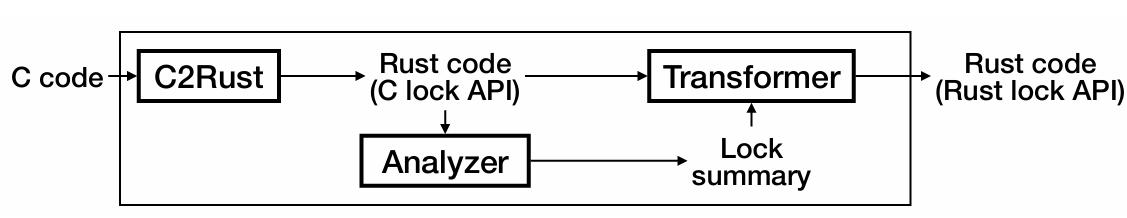
\includegraphics[width=0.8\textwidth]{ch2/assets/concratworkflow.jpg}
\decoRule
\caption[Concrat]{Concrat workflow \parencite{hong2023improving}}
\label{fig:Concrat}
\end{figure}

\break

The tool achieved valid compilable Rust code in 29 of 46 cases collected from the github, 
proving that ownership-based concurrency can be automated even for legacy codebases \parencite{hong2023improving}.
From the 46 cases, 5 of them were also compilable but with a need of a manual fixes. The remain 12 cases were considered failures
classified into three categories:  functions conditionally acquiring locks, function pointers, and pointers to locks \parencite{hong2023improving}.

Concrat focuses on C rather than C++, although its findings are applicable at C++ and also applicable to Boost C++ migration.
Libraries as Boost.Thread and Boost.Asio have a strong dependency on manual synchronization, raw pointers 
and complex ownership patterns. The study has demonstrated that a simple translation of that code to Rust, relying on C2Rust 
or C++ bindings, would preserve the safety risks unless concurrency semantics are explicitly reconstructed.
Concrat's static analysis offers a practical blueprint for the reconstruction providing a lock analysis.

This case study illustrates how automated, semantics-aware transformation can bridge the gap between C++’s flexible 
but unsafe concurrency model and Rust’s strict, verifiable approach, enabling incremental and safer integration 
of Rust into existing C++ ecosystems.

\subsection{“Just Use Rust”: A Best-Case Historical Study of Open Source Vulnerabilities in C}

In this paper the authors provide a historical security analysis of C language projects, based on the most common vulnerabilities
of C and provide answers Rust based for those vulnerabilities. Those vulnerabilities were divide into two groups: the vulnerabilities
Rust could prevent and the vulnerabilities Rust cannot prevent. Within this paper 68 prominent open source projects, as linux 
kernel and Curl, were analyzed in order to map the vulnerabilities. 

The study identified a total of 4,507 vulnerabilities across these projects, 2,257 of which had specific 
Common Weakness Enumeration \gls{CWE} designations. These were mapped to Rust's safety guarantees to determine preventative potential. 
The analysis reveals that a significant majority of historical security issues in C are memory safety errors that 
Rust effectively eliminates at compile time.

\break

\begin{figure}
\centering
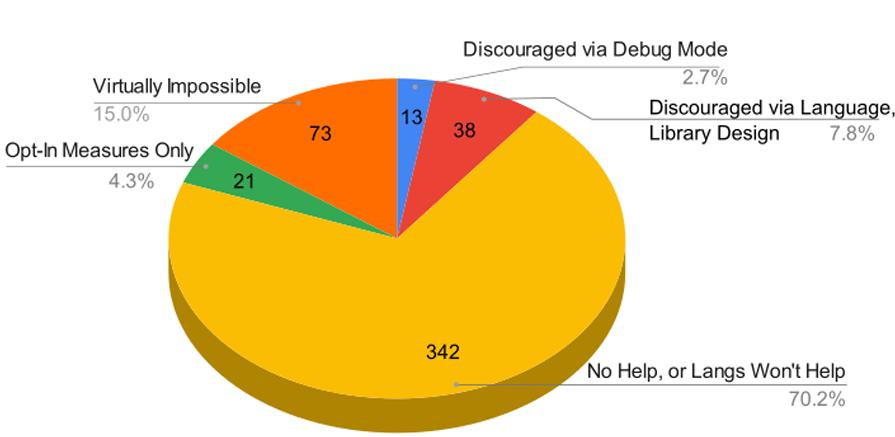
\includegraphics[width=0.8\textwidth]{ch2/assets/rustpreventions.jpg}
\decoRule
\caption[rustpreventions]{Rust Preventions based on \gls{CWE} \parencite{meneely2025just}}
\label{fig:rustpreventions}
\end{figure}

\break

As illustrated in Figure \ref{fig:rustpreventions}, the vulnerabilities are distributed across several categories of potential prevention through Rust. 
Approximately 15.0\% fall into the "Virtually Impossible" category, indicating vulnerabilities that can be prevented by 
Rust's type system and ownership model. In contrast, approximately 70.2\% fall into the "No Help, or Langs Won't Help" category, 
indicating vulnerabilities that cannot be prevented solely through the choice of programming language. 
The remaining vulnerabilities fall into intermediate categories where prevention depends on language features, libraries, 
compiler configurations, or development practices \parencite{meneely2025just}.

Table 1 details the top 20 most common vulnerability types found in the subject projects. 
The data confirms that the two most frequent issues, NULL Pointer Dereference (CWE-476) and Use After Free (CWE-416), 
accounting for nearly 17\% of all analyzed CVEs, are completely preventable in safe Rust \parencite{meneely2025just}.

\break

\begin{table}[h]
\centering
\label{tab:vulnerabilities}
% X column automatically wraps text to fit width
\begin{tabularx}{\textwidth}{|l|X|c|c|l|}
\hline
\textbf{CWE ID} & \textbf{Vulnerability Name} & \textbf{\# CVEs} & \textbf{\# Proj} & \textbf{Rust Prevention} \\ \hline
CWE-476 & NULL Pointer Dereference & 411 & 17 & Virtually Impossible \\ \hline
CWE-416 & Use After Free & 343 & 17 & Virtually Impossible \\ \hline
CWE-125 & Out-of-bounds Read & 145 & 14 & Virtually Impossible \\ \hline
CWE-20 & Improper Input Validation & 105 & 17 & No Help \\ \hline
CWE-190 & Integer Overflow or Wraparound & 100 & 12 & Discouraged (Debug) \\ \hline
CWE-401 & Memory Leak & 96 & 6 & Virtually Impossible \\ \hline
CWE-787 & Out-of-bounds Write & 92 & 15 & Virtually Impossible \\ \hline
CWE-667 & Improper Locking & 86 & 4 & Opt-In Measures \\ \hline
CWE-369 & Divide By Zero & 78 & 4 & Virtually Impossible \\ \hline
CWE-617 & Reachable Assertion & 63 & 6 & Discouraged (Debug) \\ \hline
CWE-362 & Race Condition & 62 & 11 & Discouraged (Design) \\ \hline
CWE-119 & Improper Buffer Restriction & 62 & 14 & Virtually Impossible \\ \hline
CWE-400 & Uncontrolled Resource Consumption & 59 & 15 & No Help \\ \hline
CWE-122 & Heap-based Buffer Overflow & 53 & 12 & Virtually Impossible \\ \hline
CWE-200 & Exposure of Sensitive Information & 45 & 11 & No Help \\ \hline
CWE-120 & Classic Buffer Overflow & 45 & 9 & Virtually Impossible \\ \hline
CWE-908 & Use of Uninitialized Resource & 35 & 5 & Virtually Impossible \\ \hline
CWE-415 & Double Free & 34 & 8 & Virtually Impossible \\ \hline
CWE-770 & Resource Allocation without Limits & 29 & 7 & No Help \\ \hline
CWE-131 & Incorrect Buffer Size Calculation & 26 & 7 & Virtually Impossible \\ \hline
\end{tabularx}
\caption{Top 20 Most Common Vulnerabilities and Rust Prevention Status \parencite{meneely2025just}}
\end{table}

This data suggests that while Rust is not a "silver bullet" for all security issues (such as input validation or logic bugs), 
its adoption could have theoretically prevented the majority of the most severe historical vulnerabilities 
found in these critical infrastructure projects \parencite{meneely2025just}.
        \chapter{Methodology and Solution Proposal}
        \label{chap:Chapter3}

        The migration of critical software infrastructure from C++ to Rust is not a
        syntactic translation exercise but a fundamental architectural transformation.
        It requires rethinking ownership, concurrency, and interface boundaries in order
        to preserve functionality while improving safety guarantees.

        As discussed in Chapter \ref{chap:Chapter2}, the so-called ``Boost Paradox''
        introduces a unique challenge: the very features that make Boost powerful—such as
        templates and metaprogramming—also hinder the applicability of automated
        interoperability tools.

        This chapter defines a structured methodology to decompose Boost-based systems
        and proposes an architectural design that incrementally bridges the safety gap
        between C++ and Rust.

        \section{Component Selection Criteria}
        \label{sec:SelectionCriteria}

        Historically, a ``big bang'' rewrite of large C++ codebases into Rust has proven
        prone to failure due to the difficulty of verifying feature parity, the
        disruption of ongoing development, and the elevated certification risk in
        safety-critical domains. Consequently, this research adopts a selective and
        incremental migration strategy.

        Boost libraries are not considered uniformly; instead, they are evaluated and
        selected based on their relevance, isolation capability, and suitability for
        automotive software architectures.

        \subsection{Automotive-Oriented Selection Rationale}

        The automotive sector has increasingly adopted open-source and modular software
        platforms to address growing system complexity and multi-vendor integration. In
        this context, several automotive manufacturers and suppliers participate in
        Eclipse Software Defined Vehicle initiatives, including Eclipse \gls{SCORE}.

        Eclipse \gls{SCORE} is an open-source automotive platform initiative focused on a shared
        foundation for software-defined vehicles and high-performance ECUs, with safety and
        standards alignment forming part of its development context \parencite{eclipse_score}. These initiatives reflect the
        realities of modern automotive development: large, heterogeneous C++ codebases,
        long product lifecycles, and strict constraints on timing, memory usage, and
        failure modes. Such characteristics render wholesale language replacement
        infeasible and reinforce the need for incremental, well-contained migration
        strategies.

        The Boost libraries selected for migration are therefore evaluated according to
        the following automotive-oriented criteria:

        \begin{itemize}
        \item \textbf{Relevance to in-vehicle software}: Preference is given to
        libraries commonly used in middleware, communication, configuration
        management, and concurrency control, which are prevalent in automotive
        Electronic Control Units (ECUs) and service-oriented vehicle architectures.

        \item \textbf{Deterministic behavior}: Libraries whose runtime behavior is
        predictable and suitable for real-time or near-real-time constraints are
        prioritized, aligning with automotive requirements for bounded latency and
        reproducible execution.

        \item \textbf{Safety and robustness}: Components that encode disciplined
        resource management or concurrency patterns (e.g., Boost.SmartPtr,
        Boost.Thread, Boost.Asio) are preferred, as they conceptually align with
        Rust’s ownership and concurrency models.

        \item \textbf{Isolation capability}: Libraries that can be encapsulated
        behind stable, well-defined interfaces are favored, allowing them to serve
        as clear boundaries for Foreign Function Interface (FFI) integration.

        \item \textbf{Industrial and ecosystem relevance}: Libraries and migration patterns
        that are meaningful for open automotive software ecosystems, including Eclipse
        \gls{SCORE}, are preferred because they provide a concrete architectural context
        for evaluating incremental interoperability and portability.
        \end{itemize}

        \subsection{Operational Selection Criteria and Assessment}
        \label{sec:selection_assessment}

        The criteria above are converted into an explicit assessment procedure so that component selection is traceable rather than based only on qualitative intuition. Each candidate is assessed against the following dimensions: automotive relevance, safety relevance, isolation capability, interoperability constraints, portability relevance, performance relevance, implementation complexity, and suitability for exposing reusable migration patterns.

        Each dimension is rated on a five-point ordinal scale, where 1 indicates low relevance to the migration objective and 5 indicates high relevance. The scale is used as a structured decision aid rather than as an objective measurement of library quality. The assessment is documented before implementation so that the selection is not driven by the implementation results.

        \begin{table}[H]
        \centering
        \renewcommand{\arraystretch}{1.2}
        \begin{tabularx}{\textwidth}{|l|c|X|}
        \hline
        \textbf{Criterion} & \textbf{Weight} & \textbf{Assessment question} \\ \hline
        Automotive relevance & 15\% & Is the functionality relevant to low-level or embedded automotive software? \\ \hline
        Safety relevance & 15\% & Does the component expose memory, representation, ownership, or other safety-relevant concerns? \\ \hline
        Isolation capability & 15\% & Can the functionality be encapsulated behind a stable interface? \\ \hline
        Interoperability relevance & 15\% & Does the component expose meaningful Rust/C++ boundary-design challenges? \\ \hline
        Portability relevance & 10\% & Does the component involve platform, compiler, representation, or architecture concerns? \\ \hline
        Performance relevance & 10\% & Can meaningful performance characteristics be evaluated experimentally? \\ \hline
        Implementation complexity & 10\% & Is the component complex enough to exercise the methodology but bounded enough for a dissertation case study? \\ \hline
        Pattern generalisability & 10\% & Does the component expose migration decisions that can be separated from library-specific details? \\ \hline
        \end{tabularx}
        \caption{Operational criteria used for Boost component selection}
        \label{tab:selection_criteria}
        \end{table}

        Applying these criteria to the selected case studies gives the following qualitative assessment. The values are included to make the selection rationale explicit; they should not be interpreted as a universal ranking of Boost libraries.

        \begin{table}[H]
        \centering
        \renewcommand{\arraystretch}{1.2}
        \begin{tabular}{|l|c|c|}
        \hline
        \textbf{Criterion} & \textbf{Boost.Align} & \textbf{Boost.Endian} \\ \hline
        Automotive relevance & 4 & 4 \\ \hline
        Safety relevance & 5 & 5 \\ \hline
        Isolation capability & 5 & 5 \\ \hline
        Interoperability relevance & 5 & 5 \\ \hline
        Portability relevance & 4 & 5 \\ \hline
        Performance relevance & 5 & 4 \\ \hline
        Implementation complexity & 4 & 4 \\ \hline
        Pattern generalisability & 5 & 5 \\ \hline
        \end{tabular}
        \caption{Qualitative assessment of the selected Boost libraries}
        \label{tab:selected_library_assessment}
        \end{table}

        The two libraries were retained because they expose complementary migration problems rather than because they represent the largest or most template-heavy Boost components. Boost.Align concentrates on alignment, allocation, raw-pointer access, SIMD, and a C++03 compatibility boundary. Boost.Endian concentrates on binary representation, fixed-width values, generic abstractions, and a higher-level C++ interoperability mechanism. Together, these characteristics expose different points in the migration design space while remaining sufficiently bounded for controlled experimentation.

        \subsection{Boost.Align and Boost.Endian as Migration Enablers}
        \label{sec:migration_enablers}

        The purpose of selecting Boost.Align and Boost.Endian is not to claim that they are representative of every complex Boost library. Instead, they are treated as \textbf{migration-enabling case studies}: each exposes a set of lower-level problems that must be solved before the methodology can be applied confidently to larger or more template-heavy components.

        Boost.Align exposes patterns for representing alignment requirements, controlling ownership of allocated memory, isolating raw-pointer operations, defining opaque interfaces, and preserving interoperability with a C++03 consumer. Its implementation consequently provides a case study for translating memory-oriented C++ abstractions into Rust while keeping the unsafe surface explicit.

        Boost.Endian exposes a different set of patterns. Its conversion, buffer, and arithmetic layers require explicit reasoning about binary representation, fixed-width types, generic abstractions, and C++ interoperability. The implementation uses these characteristics to investigate how semantic behaviour can be retained without reproducing the original C++ template hierarchy literally.

        The resulting contribution is therefore the identification and evaluation of migration patterns rather than a claim that these two libraries solve the general Boost migration problem. The patterns that are potentially reusable include semantic rather than syntactic translation, explicit ownership contracts, isolation of unsafe operations, minimal FFI surfaces, and compatibility-driven selection of the interoperability mechanism. Decisions such as 32-byte alignment for the evaluated AVX workload or the use of a C ABI to preserve C++03 compatibility remain case-specific.

        \subsection{Deprioritized Components}

        Not all Boost libraries are suitable for migration or interoperability with
        Rust. Libraries that rely heavily on advanced template metaprogramming,
        domain-specific embedded languages, or extensive compile-time code generation
        are deprioritized due to their limited analyzability and poor suitability for
        FFI-based integration.

        Similarly, libraries without a clear connection to the low-level concerns
        exercised by the automotive case-study context are not prioritized within the
        scope of this work. Eclipse \gls{SCORE} is used as a motivating ecosystem rather
        than as evidence that the selected Boost libraries are already used by S-CORE.

        \subsection{Safety-Critical Constraints and ISO 26262 Alignment}

        ISO-26262 requires that software architectures for automotive safety systems
        support freedom from interference, predictable execution, and systematic fault
        avoidance. Programming languages and libraries used in such systems must
        minimize undefined behavior, provide explicit ownership semantics, and enable
        static verification wherever possible \parencite{iso26262}.

        C++’s permissive memory model and reliance on developer discipline pose
        challenges when targeting higher \gls{ASIL} levels. In practice, Boost libraries
        are frequently employed in automotive systems to impose structure and
        consistency on C++ development, particularly in resource management,
        concurrency, and asynchronous communication \parencite{synopsys_asil}.

        The proposed methodology leverages this disciplined use of Boost as a
        preparatory step toward Rust integration. By constraining C++ systems to
        well-defined Boost abstractions, reliance on raw pointers, implicit ownership
        conventions, and ad hoc concurrency mechanisms is reduced. This aligns with
        ISO-26262 recommendations for limiting systematic faults through controlled
        language subsets, coding guidelines, and architectural enforcement
        \parencite{iso26262}.

        Rust components introduced under this methodology are designed to maximize the use of Rust's static ownership and type guarantees. Where unsafe operations are necessary, they are isolated, documented, and treated as explicit safety-relevant boundaries. The methodology supports safety analysis and auditability, but the dissertation does not claim certification or a complete safety case.

        \subsection{Boost Libraries Relevant to Eclipse \gls{SCORE}}

        In Eclipse \gls{SCORE}-style automotive architectures, Boost libraries are
        commonly used to support middleware services, configuration management,
        concurrency, and asynchronous I/O. Their selection is driven by the need to
        enforce structure and predictability in large-scale, safety-relevant C++
        systems.

        Table~\ref{tab:boost_score_rust} summarizes Boost libraries commonly applicable
        to automotive platforms such as Eclipse \gls{SCORE} and their corresponding
        Rust-native equivalents.

        \begin{table}[h!]
        \centering
        \begin{tabular}{|l|l|p{6cm}|}
        \hline
        \textbf{Boost Library} & \textbf{Rust Equivalent} & \textbf{Automotive Relevance} \\ \hline

        Boost.Asio &
        \texttt{tokio}, \texttt{async-std} &
        Asynchronous I/O and event handling for in-vehicle services and middleware; requires careful runtime integration in safety-critical contexts \\ \hline

        Boost.Thread &
        \texttt{std::thread}, \texttt{crossbeam} &
        Thread management and synchronization for concurrent ECU software components \\ \hline

        Boost.SmartPtr &
        \texttt{Box}, \texttt{Rc}, \texttt{Arc} &
        Explicit ownership and lifetime management; directly maps to Rust’s ownership model \\ \hline

        Boost.Optional &
        \texttt{Option\textless T\textgreater} &
        Explicit representation of optional values, reducing NULL pointer usage \\ \hline

        Boost.Variant &
        \texttt{enum} &
        Type-safe sum types used in configuration, messaging, and state machines \\ \hline

        Boost.Program\_options &
        \texttt{clap}, \texttt{argh} &
        Configuration parsing for tooling and non-safety-critical control components \\ \hline

        Boost.Filesystem &
        \texttt{std::fs}, \texttt{std::path} &
        File and path handling in diagnostic, logging, and update subsystems \\ \hline

        Boost.Chrono &
        \texttt{std::time} &
        Time measurement and timeout handling with deterministic semantics \\ \hline

        \end{tabular}
        \caption{Boost libraries relevant to Eclipse SCORE–style automotive systems and Rust equivalents}
        \label{tab:boost_score_rust}
        \end{table}

        This mapping highlights that several Boost libraries already encode concepts
        such as explicit ownership, variant-based state, and structured concurrency—
        concepts that are native to Rust. As a result, the primary challenge of
        migration is architectural rather than conceptual, reinforcing the feasibility
        of incremental Rust adoption in safety-critical automotive ecosystems.

        \subsection{Comparative Analysis as a Migration Enabler}

        A central step in the proposed methodology is the comparison between Boost
        libraries used in automotive systems and their Rust-native equivalents. This
        comparison is not a simple replacement exercise, but an architectural analysis
        that exposes semantic gaps, safety assumptions, and ecosystem limitations.

        By explicitly mapping Boost abstractions to Rust constructs, developers can:
        \begin{itemize}
        \item Identify which safety properties are already enforced at the type level
        \item Detect mismatches in ownership, error handling, or concurrency semantics
        \item Quantify the residual risk that remains after migration
        \end{itemize}

        This analysis also reveals areas where no suitable Rust equivalent exists for
        automotive-grade use. In such cases, the absence of a mature Rust library becomes
        an explicit design signal rather than an implementation obstacle.

        \subsection{From Library Gaps to New Rust Automotive Crates}
        \label{subsec:NewRustLibraries}

        The comparison between Boost and Rust ecosystems frequently uncovers
        functionality that is either missing or insufficiently mature in Rust for
        safety-critical automotive contexts.

        Rather than forcing unsafe bindings or retaining C++ dependencies indefinitely,
        the proposed methodology treats these gaps as opportunities for new Rust library
        development. Such libraries are designed from the outset with:
        \begin{itemize}
        \item Explicit ownership and lifetime semantics
        \item Deterministic execution models suitable for real-time analysis
        \item Minimal and auditable unsafe code
        \item Alignment with AUTOSAR Adaptive concepts
        \end{itemize}

        In this sense, Boost serves not only as a migration bridge, but also as a
        functional benchmark that informs the evolution of Rust’s automotive ecosystem.
        The migration process thus becomes bidirectional: existing C++ designs guide
        Rust library development, while Rust’s guarantees inform safer architectural
        patterns in C++.

        \subsection{\gls{ASIL}-Oriented Migration Strategy}

        ISO-26262 distinguishes software components according to their
        \gls{ASIL}, ranging from \gls{QM} to \gls{ASIL}-D. Each level imposes increasing
        requirements on fault avoidance, fault detection, and freedom from interference.
        As a result, a uniform migration strategy is neither practical nor desirable
        across all \gls{ASIL} levels.

        The proposed methodology adopts a differentiated migration approach:

        \begin{itemize}
        \item \textbf{QM and \gls{ASIL}-A components}: Tooling, diagnostics, logging,
        configuration services, and non-safety-critical middleware. These components
        are suitable early candidates for Rust adoption, as certification
        constraints are less restrictive.

        \item \textbf{\gls{ASIL}-B and \gls{ASIL}-C components}: Communication services, resource
        managers, and coordination logic. Rust integration at this level focuses on
        reducing the exposure to memory-safety defects while evaluating execution-time behaviour.
        Unsafe Rust is strictly isolated and subject to additional verification.

        \item \textbf{\gls{ASIL}-D components}: Rust is introduced only where its guarantees
        provide demonstrable safety benefits. Components must be ownership-complete,
        free from dynamic allocation where required, and analyzable under
        \gls{WCET} constraints. \gls{FFI} boundaries are minimized and treated as
        safety-relevant interfaces subject to rigorous review.
        \end{itemize}

        This stratification aligns with ISO-26262 recommendations for mixed-criticality
        systems and supports freedom from interference between software elements of
        different ASIL levels.


        \subsection{Migration Workflow Overview}

        Figure \ref{fig:migration_workflow} presents the proposed incremental migration
        workflow for integrating Rust into Boost-based automotive software systems.
        The workflow is designed to support safety-critical development under
        ISO-26262 constraints while preserving system continuity and certification
        traceability.

        The process begins with a \textbf{comparative analysis} of existing Boost
        library usage and available Rust-native equivalents. This step establishes a
        semantic baseline by identifying ownership models, concurrency assumptions,
        error-handling mechanisms, and determinism properties already enforced in the
        C++ architecture.

        Based on this analysis, an \textbf{architectural refactoring phase} follows,
        during which Boost abstractions are used to constrain C++ components into
        well-defined, analyzable interfaces. This step reduces semantic ambiguity,
        limits undefined behavior, and prepares the system for language boundary
        introduction without altering functional behavior.

        Next, \textbf{\gls{FFI} boundary definition} is performed. Stable and minimal
        interfaces are identified between C++ and Rust components, with explicit
        ownership transfer rules and data lifetime guarantees. These boundaries are
        treated as safety-relevant interfaces and are subject to additional review
        and verification.

        The workflow then proceeds with \textbf{incremental Rust integration}, where
        Rust components are introduced selectively according to their assigned
        \gls{ASIL} level. Initial integration targets QM and ASIL-A components, followed
        by progressively higher-criticality elements as confidence, tooling maturity,
        and safety argumentation evolve.

        Throughout the process, \textbf{continuous verification and validation} are
        performed to ensure functional equivalence, timing predictability, and freedom
        from interference. Feedback from each iteration informs subsequent migration
        steps, allowing the workflow to adapt to architectural constraints and
        certification requirements.

        \begin{figure}[h!]
        \centering
        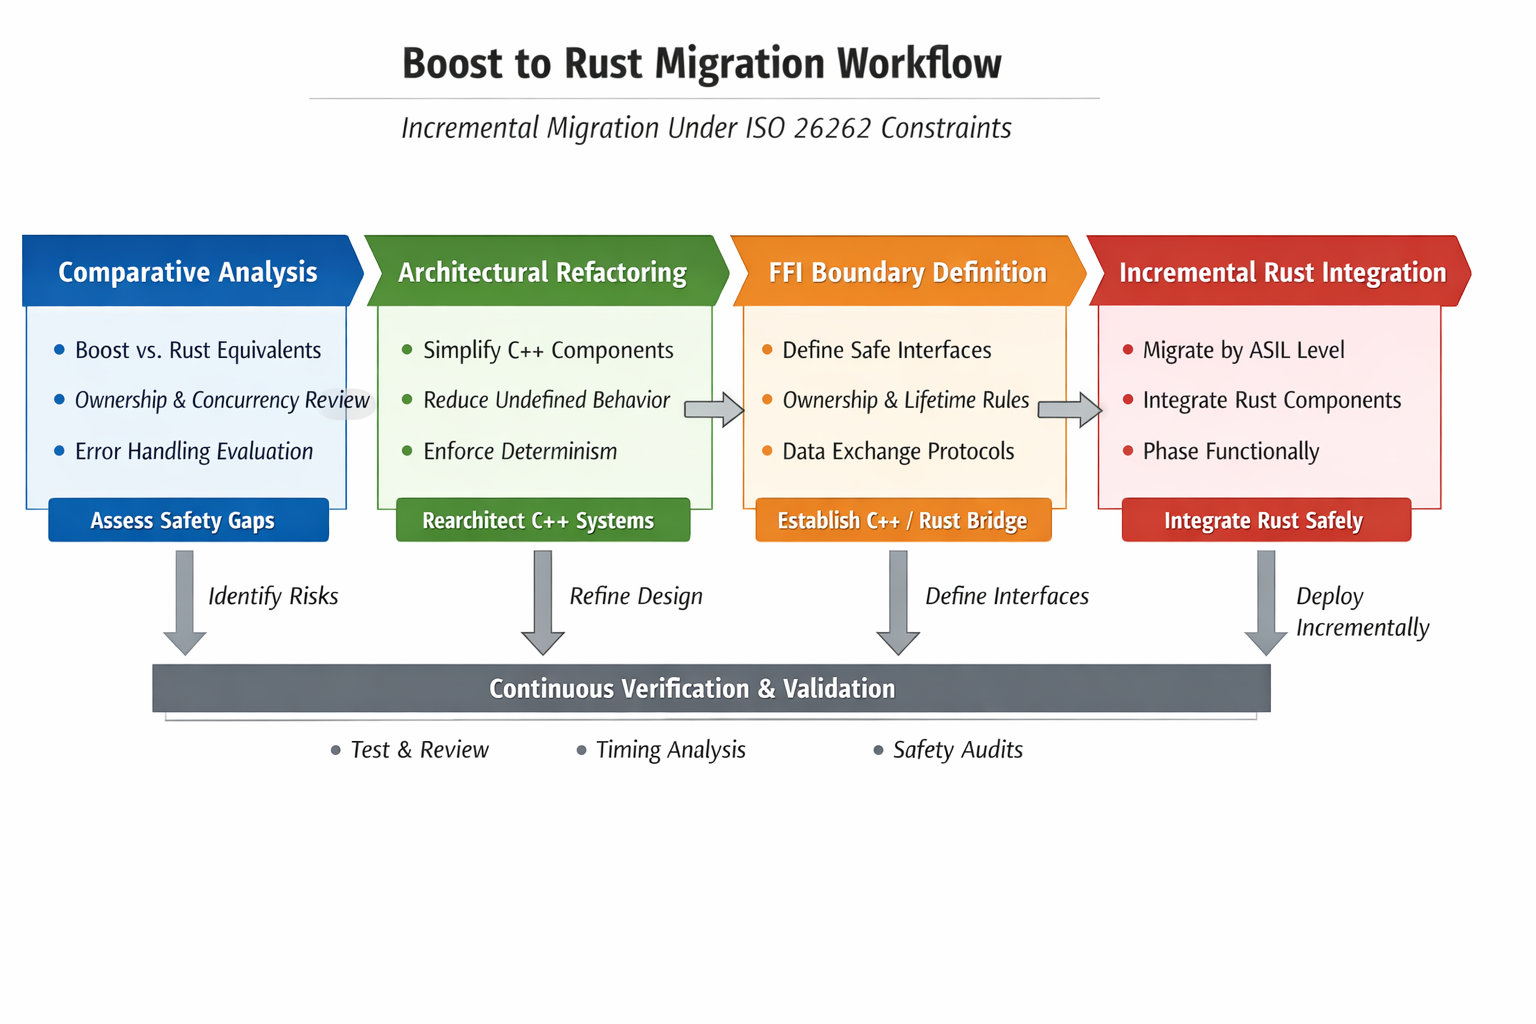
\includegraphics[width=0.9\textwidth]{ch3/assets/migration_workflow.png}
        \decoRule
        \caption[Boost-to-Rust Migration Workflow]{Incremental migration workflow for
        Boost-based automotive systems integrating Rust under ISO-26262 constraints}
        \label{fig:migration_workflow}
        \end{figure}

        Overall, the workflow emphasizes early reduction of semantic ambiguity on the
        C++ side and controlled introduction of Rust components, providing a more explicit
        interoperability boundary. Any claim of automotive safety compliance remains
        dependent on the complete system, development process, and applicable safety case.

\section{Research Design and Evaluation Plan}
\label{sec:research_design}

The proposed methodology is evaluated through two bounded case studies, \texttt{Boost.Align}
and \texttt{Boost.Endian}. The case-study design is intended to provide evidence about the
migration patterns identified by the methodology without implying that the results are
general measurements for all Boost libraries or all automotive software.

\subsection{Research Design}

Each case study follows the same high-level sequence: analysis of the original Boost
functionality, definition of equivalent Rust abstractions, implementation of the selected
functionality, integration through an appropriate FFI mechanism, functional validation,
and performance evaluation. This common structure makes it possible to distinguish
migration decisions that arise from the general methodology from those that are specific
to a library.

Boost.Align is used to evaluate low-level memory alignment, allocation, pointer handling,
SIMD-related operations, and compatibility with a C++03 consumer. Boost.Endian is used to
evaluate binary representation, fixed-width values, generic abstractions, and C++/Rust
interoperability through a higher-level interface. The two cases therefore exercise
complementary migration concerns while remaining sufficiently bounded for controlled
experimentation.

The automotive relevance is motivated by the requirements of modern software-defined
vehicle platforms. Eclipse S-CORE is an open-source automotive software platform aimed at
providing a shared foundation for high-performance ECUs and safety-critical vehicle
software, with emphasis on interoperability, portability, and automotive standards
\parencite{eclipse_score}. In this context, the selected libraries are not presented as
components that must be migrated in S-CORE itself. Instead, S-CORE is used as a motivating
architectural context in which incremental migration of low-level C++ infrastructure can
be relevant. The case studies consequently act as migration enablers: they expose
alignment, representation, ownership, and FFI patterns that can later inform work on
larger and more template-intensive components.

\subsection{Development Workflow}

The implementation follows four methodological phases: analysis; design and
implementation; interoperability; and validation and evaluation. The first phase
establishes the semantic baseline of the Boost implementation and identifies relevant
interfaces, ownership assumptions, dependencies, and observable behaviour. The second
phase defines Rust-native abstractions and implements the selected functionality without
requiring a literal translation of the C++ structure. The interoperability phase exposes
only the interface required by the existing C++ consumer. The final phase validates
functional behaviour and evaluates the measured characteristics of the resulting
implementation.

This workflow deliberately separates the conceptual methodology from the implementation
of each case study. The detailed migration procedure used within these phases is described
in Chapter~\ref{chap:Chapter4}, while the implementation and experimental results are
presented in Chapter~\ref{chap:Chapter6}.

\subsection{Validation and Evaluation Strategy}

Validation combines functional tests, interoperability checks, and benchmark measurements.
Functional validation verifies that the selected Rust functionality produces the expected
results for the evaluated inputs. Interoperability validation verifies that the exposed
interfaces can be consumed from the corresponding C++ environment. Performance evaluation
measures execution time and throughput for the workloads defined for each case study.

The evaluation is intentionally interpreted as experimental evidence for the selected
workloads. It does not establish worst-case execution time (WCET), jitter bounds,
schedulability, hard real-time guarantees, or a complete ISO 26262 safety case. Likewise,
process-level memory measurements are treated as observations of the benchmark process,
not as proof of lower memory consumption in general.

\subsection{Experimental Configuration}

The experiments use Rust 1.93 and Boost 1.91.0 as the implementation and reference
environments, respectively. Boost.Align is evaluated against a C++03-compatible interface,
while Boost.Endian uses the C++ interoperability mechanism selected for its implementation.
The benchmark configurations use release builds and repeated measurements; the reported
results are presented with the exact workload parameters in Chapter~\ref{chap:Chapter6}.

The evaluation focuses on three evidence categories: functional equivalence, measured
performance, and interoperability/safety-boundary characteristics. These categories are
sufficient to assess the feasibility of the proposed migration patterns while avoiding
claims that would require broader system-level experiments.

\subsection{Evaluation Scope and Limitations}

The selected case studies represent only a subset of Boost functionality. The results are
therefore used to evaluate the migration approach and identify practical trade-offs rather
than to generalize performance or safety properties to the complete Boost ecosystem.
In particular, the evaluation does not include complete vehicle-level integration,
long-duration operational testing, WCET analysis, multicore scheduling analysis, formal
verification, or certification assessment. These limitations are considered explicitly
when interpreting the results and the research questions in Chapter~\ref{chap:Chapter7}.


\chapter{Development Plan}
\label{chap:Chapter4}

This chapter presents the development plan for the proposed Boost-to-Rust
migration methodology. It details the planned reimplementation of selected
components in Rust, the design of stable interfaces, and the integration of
bidirectional \gls{FFI}. The plan is structured to
support incremental adoption while maintaining compliance with automotive
safety standards such as ISO-26262 and architectural principles from
AUTOSAR Adaptive.

The development activities are scheduled between February and July and are
organized to progressively reduce technical risk while preserving functional
continuity of the existing C++ system.

\section{Objectives and Scope}

The primary objectives of this development phase are:

\begin{itemize}
    \item To reimplement selected Boost-based components in Rust with equivalent
    functionality and improved memory-safety guarantees.
    \item To design explicit, minimal, and auditable interfaces between C++ and
    Rust components.
    \item To integrate Rust modules incrementally using bidirectional \gls{FFI},
    preserving deterministic behavior and freedom from interference.
    \item To validate the resulting hybrid system against safety, correctness,
    and performance expectations relevant to automotive software.
\end{itemize}

The scope of this chapter is limited to architectural and integration-level
development. Functional feature expansion beyond parity with the existing C++
implementation is explicitly excluded.

\section{Development Phases Overview}

The development plan is divided into six sequential phases:

\begin{enumerate}
    \item System analysis and Boost component selection
    \item Architectural refactoring and interface definition
    \item Rust reimplementation of selected components
    \item Bidirectional \gls{FFI} integration
    \item Validation and safety analysis
    \item Consolidation and documentation
\end{enumerate}

Each phase produces concrete artifacts that serve as inputs for the subsequent
phase, enabling traceability and controlled progression consistent with
ISO-26262 development practices.

\section{System Analysis and Component Selection}

\subsection*{February}

The initial phase focuses on analyzing the existing C++ system and identifying
Boost libraries that are relevant to automotive software architectures such as
those used in Eclipse SCORE–based environments.

The analysis includes:
\begin{itemize}
    \item Identification of Boost libraries in use and their functional roles
    \item Classification of components by criticality and \gls{ASIL} level
    \item Mapping of Boost abstractions to potential Rust-native equivalents
\end{itemize}

This phase establishes the baseline architecture and defines the migration
targets for subsequent development.

\section{Architectural Refactoring and Interface Design}

\subsection*{March}

In this phase, the selected C++ components are refactored to reduce semantic
ambiguity and prepare them for interoperability. Boost abstractions are used to
replace raw pointers, ad hoc ownership conventions, and implicit lifetimes.

Key activities include:
\begin{itemize}
    \item Encapsulation of migrated components behind stable interfaces
    \item Elimination of undefined behavior patterns
    \item Definition of ownership and lifetime semantics at component boundaries
\end{itemize}

This refactoring step does not change observable behavior but improves
analyzability and safety argumentation.

\section{Rust Reimplementation}

\subsection*{April}

During this phase, selected Boost-based components are reimplemented in Rust.
The Rust implementations are designed to be ownership-complete and memory-safe
by construction.

Design constraints include:
\begin{itemize}
    \item Explicit ownership and borrowing semantics
    \item Deterministic execution suitable for timing analysis
    \item Minimal use of \texttt{unsafe} code, isolated and documented
\end{itemize}

Functional equivalence with the original C++ components is verified through
unit testing and interface-level validation.

\section{Bidirectional \gls{FFI} Integration}

\subsection*{May}

This phase introduces bidirectional \gls{FFI} integration between C++ and Rust.
Stable C-compatible interfaces are defined, and responsibility for memory
allocation, ownership transfer, and error handling is made explicit.

Key concerns addressed include:
\begin{itemize}
    \item Isolation of unsafe code at \gls{FFI} boundaries
    \item Prevention of exception and panic propagation across language borders
    \item Alignment with AUTOSAR Adaptive service-oriented communication models
\end{itemize}

The \gls{FFI} boundary is treated as a safety-relevant interface and is subject to
additional review.

\section{Validation and Safety Analysis}

\subsection*{June}

Validation activities focus on ensuring that the hybrid C++/Rust system meets
functional, safety, and performance expectations.

This includes:
\begin{itemize}
    \item Functional regression testing
    \item Concurrency and race-condition analysis
    \item Review of freedom from interference between components of different
    \gls{ASIL} levels
\end{itemize}

The results of this phase support the safety argumentation required for
ISO-26262 compliant systems.

\section{Consolidation and Documentation}

\subsection*{July}

The final phase consolidates the development results and prepares the system
for evaluation and reporting.

Activities include:
\begin{itemize}
    \item Final architectural documentation
    \item Evaluation of migration feasibility and limitations
    \item Documentation of lessons learned and future work
\end{itemize}

This phase ensures that the development process and outcomes are reproducible
and auditable.

\section{Development Timeline}

Table \ref{tab:development_gantt} presents a Gantt-style overview of
the development plan covering the February--September period. The
activities are intentionally overlapping to reflect the iterative
nature of the migration process.

\begin{table}[H]

\centering

\renewcommand{\arraystretch}{1.3}

\begin{tabular}{|l|c|c|c|c|c|c|c|c|}

\hline

\textbf{Activity / Month} &
\textbf{Feb} &
\textbf{Mar} &
\textbf{Apr} &
\textbf{May} &
\textbf{Jun} &
\textbf{Jul} &
\textbf{Aug} &
\textbf{Sep} \\ \hline

System Analysis and Boost Selection
    & X & X &   &   &   &   &   &   \\ \hline

Architectural Refactoring and Interface Design
    &   & X & X &   &   &   &   &   \\ \hline

Rust Reimplementation
    &   &   & X & X &   &   &   &   \\ \hline

Bidirectional \gls{FFI} Integration
    &   &   &   & X & X &   &   &   \\ \hline

Validation and Safety Analysis
    &   &   &   &   & X & X & X &   \\ \hline

Performance Evaluation and Optimization
    &   &   &   &   &   & X & X &   \\ \hline

Consolidation and Documentation
    &   &   &   &   &   &   & X & X \\ \hline

Final Evaluation and Reporting
    &   &   &   &   &   &   &   & X \\ \hline

\end{tabular}

\caption{Gantt-style development plan for the Boost-to-Rust migration}

\label{tab:development_gantt}

\end{table}

\chapter{Migration strategy}
\label{chap:Chapter5}

This chapter defines a systematic strategy for migrating selected Boost libraries to Rust.
The strategy establishes a common methodology that is applicable to each of the selected libraries and provides
a structured approach for evaluating the resulting implementations.

The primary objective of the proposed strategy is to reproduce the relevant functionality of the selected Boost libraries in Rust 
while preserving their expected behavior and enabling their integration with existing C++ codebases. In addition, the strategy 
considers the requirements and constraints associated with the potential use of the migrated libraries in safety-critical 
automotive software architectures.

The migration strategy is divided into six main steps, described below:
\begin{enumerate}
\item \textbf{Understanding the library's functionality and its dependencies.}

The first step consists of analyzing the selected Boost library's source code, documentation and 
relevant technical literature, to understand its purpose, functionality, interfaces and dependencies.

This analysis identifies the relevant classes,funtions, data structures, algorithms, platform-specific
behavior and interactions with other libraries.
Particular attention is given to aspects that affect the observable behavior of the library and that may influence its migration to Rust.

A comprehensive understanding of these aspects is essential to ensure that the Rust implementation reproduces the relevant
semantics of the original library and can be subsequently be integrated into existing C++ codebases.

\item \textbf{Define Rust equivalents for the library's classes, functions, and data structures.}

Based on the analysus of the library's original implementation, the equivalent Rust abstractions
are defined for the library's classes, functions, data structures and interfaces. 

The Rust design does not necessarily replicate the structure of the original C++ implementation. 
Where appropriate, the design may differ in order to take advantage of Rust's ownership model,
type system, error handling mechanisms and idiomatic programmig practices, while preserving the required behavior of the original library.

\item \textbf{Implement the library's functionality in Rust, ensuring that it adheres to Rust's memory safety guarantees 
and best practices.}

The library's functionality is reimplemented in Rust. During this stage, particular attention is given to the Rust's ownership
and borrowing model, memory safety guarantees, error handling and idiomatic design principles. 

The implemenentation also considers the requirements and constraints of intended target environment.
Where the use of \texttt{unsafe} Rust is necessary, such usage should be minimized and restricted to well-defined boundaries, 
particularly when interacting with external code or platform-specific functionality.

\item \textbf{Create a C++ wrapper for the Rust implementation, allowing it to be used in existing C++ codebases.}

To enable integration with existing C++ codebases, an interoperability layer (C++ wrapper) is developed around the Rust implementation. 

The interoperability layer provides an interface suitable for use by the existing C++ applications while isolating the 
underlying Rust implementation from the consuming code.
Particular attention is given to the representation of data, ownership and object lifetime, error handling, memory management and 
the interaction between the C++ and Rust components.

\item \textbf{Test the Rust implementation and the C++ wrapper to ensure that they function correctly 
and meet performance requirements.}

The Rust implementation and its C++ wrapper are tested to verify functional correctness, behavioral equivalence with the original
Boost library where applicable, interoperability and performance. 

The original Boost implementation serves as a reference when behavioral compatibility is required. 
Equivalent inputs and relevant execution scenarios are used to identify discrepancies between the original and migrated implementations.

Performance evaluation is also performed to determine whether the Rust implementation and the 
interoperability layer introduce unacceptable overhead compared with the original implementation.

\item \textbf{Document the migration process, including any challenges encountered and solutions implemented, 
to provide guidance for future migrations of other Boost libraries to Rust.}

The final step consists of documenting the migration process, including design decisions, encoutered challenges, solutions, 
testing results and lessons learned. 

This documentation provides a reference for future migrations to other Boost libraries and 
contributes to the definition of a repeatable migration methodology.

\end{enumerate}

Among these steps, two are particularly critical for the success of the migration strategy. The first is the {analysis of 
the library's functionality and dependencies}, since an incomplete understanding of the original implementation can result in 
incorrect assumptions about its behavior or dependencies. The second is the \textbf{implementation of the functionality in Rust}, 
as this stage requires translating the original C++ abstractions into Rust while preserving the required semantics and taking 
advantage of Rust's memory safety guarantees and type system. These two stages therefore have a significant influence on the 
correctness and overall sucess of the migration.

\begin{figure}[H]
\centering
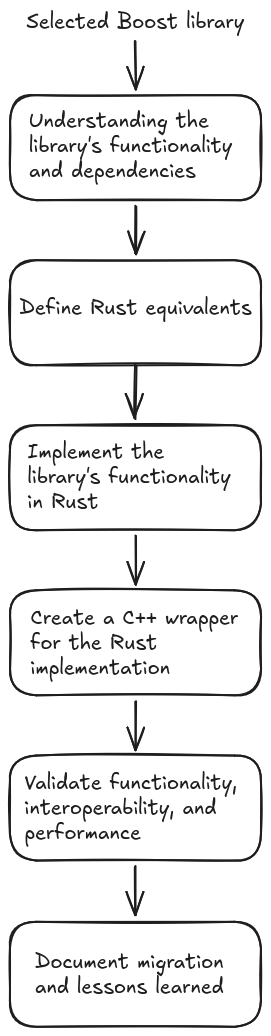
\includegraphics[width=0.25\textwidth]{ch5/assets/strategy.png}
\decoRule
\caption[Strategy]{Migration strategy}
\label{fig:Strategy}
\end{figure}

\newpage

The six steps described above can be grouped into four main phases, as follows:

\begin{enumerate}
\item \textbf{Analysis}
\begin{enumerate}
\item Understanding the library's functionality and dependencies.
\item Defining the migration scope and requirements.
\end{enumerate}
\item \textbf{Design and Implementation}
\begin{enumerate}
\item Defining the Rust equivalents of the relevant C++ abstractions.
\item Implementing the required functionality in Rust.
\end{enumerate}
\item \textbf{Interoperability}
\begin{enumerate}
\item Developing the interoperability layer between Rust and C++.
\end{enumerate}
\item \textbf{Validation and Evaluation}
\begin{enumerate}
\item Testing functional correctness, behavioral equivalence, interoperability, and performance.
\item Documenting the results, limitations, and lessons learned.
\end{enumerate}
\end{enumerate}

The phases are illustrated in Figure \ref{fig:Phases}.

\begin{figure}[H]
\centering
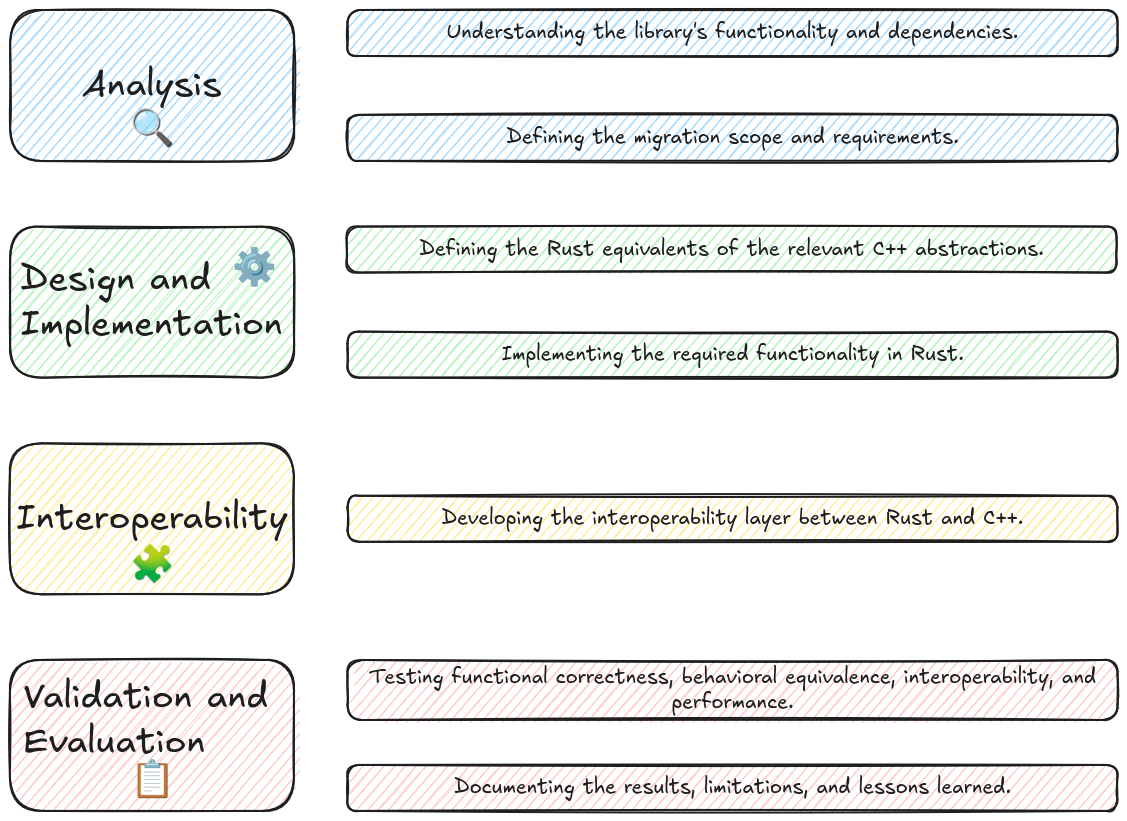
\includegraphics[width=0.8\textwidth]{ch5/assets/phases.png}
\decoRule
\caption{Migration phases}
\label{fig:Phases}
\end{figure}

\newpage

The migration strategy aims to satisfy the following objectives:

\begin{itemize}
\item Preserve the relevant behavior of the original Boost library;
\item Provide equivalent functionality through a Rust implementation;
\item Maintain interoperability with existing C++ applications;
\item Leverage Rust's memory and type safety guarantees;
\item Maintain acceptable performance compared with the original implementation;
\item Minimize and isolate the use of \texttt{unsafe} Rust, particularly at interoperability boundaries;
\item Consider the requirements and constraints of the intended automotive environment.
\end{itemize}

The success of a migration is therefore evaluated according to the extent to which these objectives are satisfied. 
The specific application of the proposed strategy, including the analysis, implementation, interoperability and 
evaluation of each selected Boost library, is presented in the following chapter.

\chapter{Selected libraries}
\label{chap:Chapter6}

This chapter presents the selected Boost libraries for reimplementation in Rust.
The selection is based on several criteria, including their relevance to automotive software architectures, implementation characteristics, 
complexity and the potential benefits that a Rust implementation may provide in terms of memory safety, reliability and performance.

The selected libraries are: \texttt{Boost.Align} and \texttt{Boost.Endian}. Both libraries provide relatively low-level functionality
that is relevant to systems programming and embedded software, while also exposing functionality that interacts closely with memory
representation and processor architecture. These characteristics make them suitable candidates for evaluating the feasibility of 
reproducing existing C++ functionality using idiomatic Rust.

For each selected library, this chapter provides an overview of its purpose and functionality, describes its main components and discusses
its relevance to automotive software development. The chapter also identifies the main challenges associated with reimplementing the library
in Rust, including differences between the C++ and Rust memory models, language abstractions, portability requirements and interoperability
with existing C++ codebases.

\section{Boost.Align}
\subsection{Overview}

The \texttt{Boost.Align} library provides functions, classes, templates, traits and macros, for controlling, inspecting and diagnosing 
memory alignment. Its primary purpose is to provide portable alignment-related functionality across different compilers, standard library
implementations and language standards.

Memory alignment refers to the requirement that an object is stored at a memory address satisfying a particular alignment constraint. 
For example, a type with an alignment requirement of 8 bytes must generally be placed at an address divisible by 8. 
Alignment requirements are determined by the target architecture and by the type being stored. 
Correct alignment is important because processors may impose restrictions on the addresses from which particular types can be accessed. 
Even on architectures that support unaligned accesses, aligned accesses can provide more predictable and efficient memory operations.

Alignment is particularly relevant to low-level and performance-sensitive software. 
Incorrectly aligned objects may result in inefficient memory accesses or, on architectures with stricter alignment requirements, hardware faults.
In C++, violating the alignment requirements of an object can also result in undefined behavior. 
Consequently, explicit control over memory alignment can be important when implementing data structures, 
custom allocators, memory pools, serialization mechanisms, and other low-level components.

Before C++ 11, the language provided limited standardized facilities for expressing and manipulating alignment requirements.
Boost.Align addressed this limitation by providing portable alignment utilities that could be used in C++03 code and 
across implementations with incomplete or inconsistent support for newer alignment-related facilities.

C++11 introduced standardized support for specifying alignment requirements through language and library facilities. 
In particular, the language introduced alignment specifications through \texttt{alignas}, 
while the standard library introduced facilities such as \texttt{std::align}. 
However, compiler and standard library support was not always complete or consistent at the time Boost.Align was developed. 
The library therefore also provided portable implementations and compatibility facilities for environments in which 
the corresponding standard functionality was unavailable or unreliable.

\subsection{Functionality}

Boost.Align provides functionality for both dynamic memory allocation and pointer alignment.
Its facilities can broadly be divided into allocation, pointer alignment, alignment inspection, and alignment diagnostics.

For dynamic memory allocation, the library provides:

\begin{itemize}
\item \texttt{aligned\_alloc(alignment, size)}, which allocates a block of memory satisfying a specified alignment requirement;
\item \texttt{aligned\_free(ptr)}, which releases memory previously allocated using the corresponding aligned allocation mechanism.
\end{itemize}

These functions are useful when the default allocation provided by the runtime or standard library does not guarantee 
the alignment required by an application or data structure.

The library also provides allocator abstractions, including:

\begin{itemize}
\item \texttt{aligned\_allocator<T>};
\item \texttt{aligned\_allocator_adaptor<Allocator>};
\item \texttt{aligned\_delete<T>}.
\end{itemize}

The allocator abstractions allow alignment requirements to be integrated with C++ allocation mechanisms and standard containers.
This is particularly useful for containers whose elements must satisfy an alignment requirement greater than 
the default alignment provided by the allocator.

Another important part of Boost.Align concerns pointer alignment.
The library provides an implementation of functionality equivalent to \texttt{std::align}, 
allowing a pointer within an available memory region to be adjusted to satisfy a requested alignment 
while preserving the required amount of available storage.

This functionality is relevant when implementing custom memory-management mechanisms.
For example, an application may reserve a larger memory region and subsequently divide it into several aligned regions for different objects.
Explicit pointer alignment allows such regions to be placed at addresses compatible with the alignment requirements of the objects they contain.

The library additionally provides facilities for querying and inspecting alignment requirements.
These capabilities allow software to determine the alignment associated with a type or address and 
to verify whether an address satisfies a particular alignment constraint. 
Such facilities are useful when implementing generic low-level components where the alignment requirements cannot be assumed statically.

\subsection{Relevance to automotive software}

Memory alignment is particularly relevant to automotive software because many automotive systems operate under strict constraints 
regarding performance, memory consumption, determinism, and hardware compatibility. Software components may interact directly with hardware, 
communication buffers, memory-mapped data, DMA regions, or specialized data structures whose layout and alignment must be carefully controlled.

For example, an automotive application may process large collections of sensor data or 
communication frames using structures with specific alignment requirements. 
Correct alignment can contribute to efficient memory accesses and may be necessary to satisfy 
the requirements of a particular processor or hardware interface.

Alignment can also become important when software is designed to run across multiple processor architectures. 
Automotive platforms may use different CPU architectures and compiler toolchains, each with potentially different alignment characteristics. 
A portable abstraction for alignment can therefore reduce the amount of platform-specific code required by a software component.

Furthermore, automotive software frequently contains legacy C++ codebases that were developed before the widespread availability 
of modern C++ standards. Such systems may continue to rely on Boost libraries to provide functionality 
that was historically unavailable or insufficiently portable in the C++ language and standard library.

Although many of the capabilities historically provided by Boost.Align are now available through modern C++ language and 
standard library facilities, Boost.Align remains relevant when maintaining or migrating legacy systems. 
Reimplementing these facilities in Rust therefore provides an opportunity 
to investigate how low-level memory-management functionality originally designed for C++ can be expressed 
using Rust's stronger type system and ownership model.

\subsection{Challenges of reimplementation in Rust}

Reimplementing Boost.Align in Rust presents several challenges. 
The most significant is the interaction between explicit memory alignment and Rust's safety guarantees.

Rust provides alignment information as part of its type system and guarantees that references 
to properly typed values satisfy the corresponding alignment requirements. 
However, operations involving raw pointers, manually allocated memory, and custom allocation strategies 
may require the use of \texttt{unsafe} code. 
Consequently, an implementation of Boost.Align-like functionality must carefully isolate unsafe operations and 
ensure that the safety invariants expected by the Rust type system are preserved.

Dynamic aligned allocation is another important consideration. 
Rust's allocation APIs allow an allocation to be described through a \texttt{Layout}, 
which contains both the size and alignment of the requested memory region. 
This provides a natural abstraction for implementing functionality similar to Boost.Align's aligned allocation mechanisms. 
Nevertheless, the implementation must correctly handle invalid layouts, allocation failures, deallocation, 
and the relationship between an allocation's size and alignment.

Pointer alignment presents an additional challenge because it requires reasoning about raw memory addresses and available storage. 
A Rust implementation must ensure that pointer arithmetic does not violate the language's safety requirements and 
that any resulting pointer is only converted into a reference when all required invariants are satisfied.

Allocator integration also differs significantly between C++ and Rust. 
Boost.Align integrates with the C++ allocator model and standard containers, 
whereas Rust uses the \texttt{GlobalAlloc} and allocator-related abstractions available in the language ecosystem. 
Therefore, a direct translation of the C++ interfaces would not necessarily result in an idiomatic Rust implementation. 
Instead, the reimplementation should preserve the observable semantics of the original library while adapting its interface to Rust's ownership, 
borrowing, and allocation abstractions.

Finally, portability must be considered. 
The original Boost library was designed to compensate for differences between compilers and standard library implementations. 
A Rust implementation should therefore be evaluated across the relevant target architectures and 
toolchains to determine whether its behavior is consistent and whether platform-specific assumptions have been introduced.

\subsection{Rationale for selection}

Boost.Align was selected because it represents a low-level library whose functionality is closely related to memory management and 
processor architecture. It therefore provides a useful case study for evaluating the migration of C++ systems-level functionality to Rust.

The library is also particularly suitable for examining the boundary between safe and unsafe Rust. 
While many high-level uses of aligned data can be expressed safely through Rust's type system, 
explicit allocation and pointer manipulation require lower-level primitives. 
This makes Boost.Align useful for assessing whether Rust can provide a safer abstraction around functionality 
that traditionally requires careful manual reasoning in C++.

In addition, Boost.Align provides a relatively compact and well-defined API while still containing several distinct concepts, 
including alignment calculation, pointer manipulation, dynamic allocation, and allocator integration. 
This provides sufficient implementation complexity to evaluate the migration methodology without making the selected library unnecessarily large.

Although alignment support has substantially improved in modern C++ and much of the functionality 
provided by Boost.Align is now represented by standard C++ facilities, 
the library remains relevant when dealing with older C++ codebases and portability requirements. 
Its reimplementation in Rust can therefore demonstrate how existing low-level C++ infrastructure can be reproduced 
while taking advantage of Rust's memory-safety guarantees and modern abstractions.

The original Boost.Align documentation and source code were used as the primary references for the analysis and subsequent reimplementation:

\begin{itemize}
\item \url{https://github.com/boostorg/align/blob/boost-1.91.0/doc/align.qbk}
\item \url{https://www.boost.org/library/latest/align/}
\item \url{https://www.boost.org/doc/libs/latest/doc/html/align.html}
\end{itemize}

\section{Boost.Endian}
\subsection{Overview}

The \texttt{Boost.Endian} library provides facilities for manipulating the byte order, or endianness, of integer and 
user-defined types. Endianness defines the order in which the individual bytes of a multi-byte value are represented in
the memory. The two predominant byte-ordering schemes are little-endian, where the least significant byte is stored 
first, and big endian, where the most significant byte is stored first.

Endianness is generally transparent to application level software when the data remains within a single system.
However, it becomes relevant when binary data is exchanged between systems, stored in files, transmitted over networks,
or interpreted by software running on different processor architectures. In such cases, the representation of a value
in memory may differ from the representation expected by the receiving system.

As example, considering a 16-bit value such as \texttt{0x0102} is represented as the byte sequence \texttt{0x01 0x02} 
on a big-endian system and as \texttt{0x02 0x01} on a little-endian system. If the byte representation 
is interpreted without considering its endianness, the received application may obtain a different numerical value, 
leading to incorrect behavior or data corruption. Consequently, explicitly defining and handling byte order 
is an important requirement for portable binary data formats and communication protocols.

Boost.Endian was developed to provide a portable and consistent abstraction for these operations. The library supports 
binary data portability independently of the native endianness of the host platform and provides a common interface
across different C++ environments. It also addresses a secondary use case involving data size optimization by 
providing integer representations with sizes that are not directly available as standard C++ integer types, 
such as 24-bit, 40-bit and 48-bit integers. These types can be useful when implementing compact binary data formats or communication protocols.

The library is header only and in its current version, requires C++11. It can make use of compiler provided byte swapping intrinsics 
when available, allowing implementations to take advantage of architecture specific instructions while retaining a portable interface.

\subsection{Functionality}

Boost.Endian provides three complementary approaches for working with endian dependent data: endian conversion functions,
endian buffer types and endian arithmetic types. Each approach is designed for a different balance between explicitness, 
ease of use, performance and control over when conversions take place.

\subsubsection{Endian conversion functions}

The conversion function approach uses the standard C++ integer types to store values and explicitly converts their representation 
when required. The library provides both mutating and non-mutating conversion operations, including unconditional and conditional variants.

For example, an application can convert a value from big endian to the native byte order before performing calculations and convert
it back before writing the value to an external representation. This approach makes the conversion points explicit and is 
particularly appropriate when an application already has an established data model based on the native C++ types.

The conversion functions also provide a relatively direct abstraction over underlying processor byte swapping operations. When compiler
intrinsics are available, Boost.Endian can use them to generate efficient machine code.

\subsubsection{Endian buffer types}

Endian buffer types store values in a representation with a specified byte order. Unlike ordinary native integer types,
the representation maintained by the buffer does not change depending on the host architecture.

The library provides buffer types for a range of integer sizes, including 8-bit, 16-bit, 24-bit, 32-bit, 40-bit, 48-bit, 56-bit
and 64-bit integers. Both aligned and unaligned representations are available, with unaligned representations being particularly
useful when dealing with tightly packed binary formats.

An important characteristic of buffer types is that the conversions are explicit. A value must be explicitly loaded from or stored
into the endian representation. This prevents hidden conversions and gives the programmer precise control over when byte order 
transformation occurs.

This property is useful for binary protocols and file formats where the in memory representation must remain stable regardless 
of the architecture on which the software is executed.

\subsubsection{Endian arithmetic types}

Endian arithmetic types combine a fixed byte-order representation with an interface similar to the built-in C++ arithmetic types. 
They support arithmetic operations while automatically performing the required conversions between the stored representation and 
the native representation.

This approach simplifies application code because explicit conversions do not have to be performed for every arithmetic operation. 
For example, an application can maintain a structure containing big-endian integer fields and operate on those fields 
using normal arithmetic expressions.

The convenience of implicit conversion comes with a potential performance trade-off. 
Repeated operations on endian arithmetic types may result in repeated conversions, particularly inside computationally intensive loops. 
Boost.Endian therefore also documents patterns for moving conversions outside performance-critical loops when necessary.

\subsection{Binary data portability}

One of the primary motivations for Boost.Endian is binary data portability. 
Binary formats frequently specify the exact byte ordering and size of their fields. Unlike textual representations, 
binary formats cannot rely on the receiving system to interpret values according to its native representation.

This is particularly important for network protocols, file formats, serialization systems, and inter-process communication mechanisms. 
A data structure containing several integer fields may have to be transmitted from a little-endian processor to another system 
whose native representation is different. 
Explicitly representing the required byte order ensures that the same logical value is reconstructed at the destination.

Boost.Endian therefore separates the representation of externally defined binary data from the native representation of the host machine. 
This allows the application to use a consistent representation for data exchanged with external systems 
while remaining independent of the processor's native byte order.

The library also supports unaligned integer representations. 
This is useful for binary formats where fields are packed without the padding that would normally be introduced by C++ object alignment. 
Boost.Endian specifically identifies unaligned 24-, 40-, 48-, and 56-bit representations as useful 
when the exact size of the external representation matters.

\subsection{Relevance to automotive software}

Endianness is particularly relevant to automotive software because modern automotive systems consist of heterogeneous hardware 
and software components that communicate using precisely defined binary data formats.

Automotive systems commonly exchange data between electronic control units, sensors, gateways, communication interfaces, 
and higher-level computing platforms. These components may use different processors, operating systems, compilers, and software stacks. 
Consequently, communication interfaces cannot generally rely on the native representation of a particular processor.

The problem becomes particularly relevant when software processes binary communication frames or serialized data structures. 
A protocol may define a field as a 16-bit or 32-bit integer with a specific byte ordering, 
independently of the architecture executing the software. 
The implementation must therefore interpret the field according to the protocol definition rather than according to the host architecture.

This characteristic makes endian handling relevant to automotive communication stacks, serialization libraries, diagnostic protocols, 
and other components operating close to hardware and communication interfaces.

The relevance of these concerns is also reflected in modern automotive software platforms. 
The Eclipse S-CORE project, for example, is an open-source initiative focused on a software-defined vehicle platform 
and provides an example of the increasing role of modern software architectures and cross-platform technologies in automotive systems.

For an automotive software architecture, using explicit endian-aware representations can therefore help establish a clear boundary 
between the internal representation of application data and the representation required by an external communication or storage format.

\subsection{Memory representation and portability}

Boost.Endian is also relevant to portability because it avoids assuming that the host architecture uses the same byte order 
as the external data source.

A naïve implementation may interpret a binary structure directly through a native C++ structure. 
Such an approach can introduce portability problems because the resulting representation can depend on the processor's endianness, 
alignment requirements, padding rules, and compiler behavior.

For example, a structure containing several native integer fields cannot necessarily be treated as a portable representation 
of a network or file format simply by writing its memory contents directly to a file or communication channel. 
The representation of the fields may differ between platforms, and additional padding may be introduced by the compiler.

Endian-aware types provide a mechanism for explicitly representing the byte order required by the external format. 
This allows the application to distinguish between the representation used for communication and the representation used 
internally for computation.

This distinction is particularly valuable in safety- and reliability-oriented systems because it makes assumptions about 
binary representation explicit rather than relying on implicit properties of the target architecture.

\subsection{Performance considerations}

Byte-order conversion is generally a low-level operation that can be implemented efficiently using processor instructions. 
Boost.Endian takes advantage of compiler intrinsics when available, including byte-swap operations provided by GCC, Clang, 
and Microsoft Visual C++.

The performance characteristics of the different Boost.Endian approaches depend on how frequently conversions occur. 
When conversion functions are used, the programmer can explicitly control when a value is converted. 
This can be advantageous when a value is used repeatedly because the conversion can be performed once before a computationally intensive 
operation and the result converted back only when necessary.

Endian arithmetic types provide greater convenience but may perform implicit conversions during arithmetic operations. 
Boost.Endian's documentation demonstrates that, particularly in repeated computations, 
explicitly controlling the location of conversions can avoid unnecessary byte swapping.

This distinction is relevant for automotive applications because software may simultaneously have strict requirements for 
portability and computational efficiency. Communication-oriented code may prioritize explicit representation and correctness, 
while performance-critical processing may require minimizing repeated conversions.

\subsection{Challenges of reimplementation in Rust}

Reimplementing Boost.Endian in Rust presents several challenges, although Rust provides several primitives that are well suited to the problem.

The first challenge is representing values with an explicitly defined byte order while maintaining Rust's type 
and memory-safety guarantees. 
Rust's standard library provides methods such as \texttt{from\_be}, \texttt{from\_le}, \texttt{to\_be}, and \texttt{to\_le}, 
as well as byte-oriented conversion facilities. These provide a strong foundation for implementing endian-aware abstractions, 
but they do not directly reproduce the complete Boost.Endian API.

A second challenge is the implementation of endian-aware buffer types. 
Such types need to preserve a specific byte representation independently of the host architecture. 
A Rust implementation can use byte arrays as the underlying representation, which has the advantage of 
making the representation explicit and avoiding direct dependence on native integer layout.

Unaligned representations introduce another challenge. Rust provides strong guarantees around references and alignment, 
meaning that interpreting an arbitrary byte sequence directly as an integer reference may require unsafe operations. 
A safe implementation should therefore prefer byte-based representations and explicit conversion operations where possible, 
isolating any required unsafe code behind a well-defined abstraction.

A further challenge is reproducing Boost.Endian's arithmetic types. Boost.Endian allows endian-aware values to 
participate directly in arithmetic expressions, while Rust's operator traits provide a different abstraction mechanism. 
Implementing equivalent behavior requires implementing traits such as \texttt{Add}, \texttt{Sub}, \texttt{Mul}, 
and their assignment variants where appropriate.

However, a direct translation of the C++ API would not necessarily produce an idiomatic Rust library. 
Rust's ownership model, trait system, explicit conversion mechanisms, and emphasis on compile-time safety provide opportunities 
to design a safer interface rather than reproducing the C++ interface exactly.

Another important consideration is floating-point support. Endianness of floating-point representations cannot always be treated as 
a simple integer byte swap because floating-point representation and byte ordering involve additional assumptions. 
Boost.Endian therefore places restrictions on some floating-point conversion operations. A Rust reimplementation must 
preserve these semantic limitations rather than assuming that arbitrary floating-point values can safely be transformed by reversing their bytes.

\subsection{Rationale for selection}

Boost.Endian was selected because it represents a particularly relevant example of low-level, 
cross-platform functionality that is commonly required when implementing systems software.

Unlike functionality that is primarily concerned with convenience abstractions, 
endian handling directly affects the representation of data exchanged between software components. 
This makes the library particularly relevant to automotive architectures, where multiple software 
and hardware components must exchange binary data according to well-defined protocols.

The library also provides an interesting migration target because it contains several distinct implementation strategies: 
conversion functions, buffer types, and arithmetic types. These approaches expose different trade-offs between explicitness, 
ease of use, memory representation, and performance. 
Reimplementing them in Rust provides an opportunity to evaluate how these design choices can be expressed using Rust's type system 
and trait-based abstractions.

The support for both aligned and unaligned representations is another reason for its selection. 
It introduces a direct connection to low-level memory representation and requires careful consideration of alignment, 
raw byte access, and safe abstractions. This complements the selection of \texttt{Boost.Align}, which focuses explicitly on memory alignment.

The combination of \texttt{Boost.Align} and \texttt{Boost.Endian} is therefore particularly useful for the migration study. 
While Boost.Align focuses on the physical placement and alignment of objects in memory, 
Boost.Endian focuses on the representation and interpretation of multi-byte values. 
Together, they cover two closely related aspects of low-level systems programming: how data is positioned in memory and 
how that data is represented across system boundaries.

Furthermore, Boost.Endian is sufficiently mature and well-defined to provide a meaningful basis for 
comparing the original C++ implementation with a Rust implementation. The library's documented performance considerations, 
multiple API approaches, and portability requirements provide several dimensions against which the Rust implementation can be evaluated.

The primary references used for the analysis are:

\begin{itemize}
\item \url{https://www.boost.org/library/latest/endian/}
\item \url{https://www.boost.org/doc/libs/latest/libs/endian/doc/html/endian.html}
\item \url{https://github.com/eclipse-score}
\end{itemize}

\chapter{Conclusions and Future Work}

\label{chap:Chapter7}

\section{Conclusions}
\label{sec:conclusions}

This dissertation investigated an incremental approach for migrating selected low-level Boost functionality from C++ to Rust while preserving interoperability with existing C++ software. The work treated migration as an architectural and semantic transformation rather than as a direct source translation. Two case studies, \texttt{Boost.Align} and \texttt{Boost.Endian}, were implemented using different interoperability strategies so that the methodology could be evaluated under different compatibility constraints.

The study demonstrates that selected functionality from both libraries can be expressed using Rust-native abstractions while retaining a usable C++ integration boundary. The implementations also show that the appropriate FFI mechanism depends on the compatibility requirements of the component: the Align implementation uses a small C-compatible interface because the target use case retains C++03 compatibility, whereas the Endian implementation uses the \texttt{cxx} bridge.

The evaluation provides quantitative evidence for the selected workloads. In the Boost.Align end-to-end benchmark, the Rust implementation measured 20.7014~ms per iteration compared with 21.6782~ms for the Boost implementation, corresponding to approximately 4.7\% lower measured execution time. The same experiment reported a larger RSS increase during allocation for the Rust implementation, so the results do not support a general claim of reduced memory consumption. In the Boost.Endian benchmark, Rust through the \texttt{cxx} bridge measured lower execution time than the manual C++ byte-manipulation baseline at all four tested input sizes, with a reported average speedup of approximately 35\%. Because that baseline is not the original Boost.Endian implementation, the result should not be interpreted as evidence that Rust is generally faster than Boost.Endian.

The central conclusion is therefore methodological: successful incremental migration depends on identifying observable semantics, selecting an appropriate Rust abstraction, defining an explicit interoperability contract, isolating unsafe operations, and validating each migrated component with evidence appropriate to the property being claimed. The two case studies demonstrate these patterns without establishing that every Boost component, particularly highly template-dependent components, can be migrated using the same implementation choices.

\section{Answers to the Research Questions}
\label{sec:answers_research_questions}

\subsection{RQ1 -- Architectural and interoperability patterns}

The implementation identifies several reusable patterns: semantic rather than syntactic translation, explicit ownership and lifetime contracts, small FFI surfaces, isolation of unsafe operations, compatibility-driven FFI selection, and validation against observable behaviour. These patterns are implemented in different forms for Align and Endian rather than through a single universal binding mechanism.

\subsection{RQ2 -- Component-selection criteria}

The methodology defines selection criteria covering automotive relevance, safety relevance, isolation capability, interoperability constraints, portability, performance relevance, implementation complexity, and the potential to expose reusable migration patterns. These criteria provide a traceable basis for selecting case studies rather than selecting components solely because they are easy to translate.

\subsection{RQ3 -- Rust reimplementation while preserving behaviour}

The two case studies demonstrate that selected Boost functionality can be re-expressed using Rust-native abstractions while preserving the tested observable behaviour. The implementations do not reproduce the complete Boost APIs or their internal C++ structures. Consequently, the evidence supports semantic reproduction of the selected functionality rather than complete API equivalence.

\subsection{RQ4 -- FFI boundary design}

The implementations show two compatible approaches. Boost.Align uses a small C-compatible boundary suitable for C++03 consumers, while Boost.Endian uses \texttt{cxx}. In both cases, interface design requires explicit reasoning about representation, ownership, lifetime, valid inputs, and error or panic behaviour. The appropriate mechanism is therefore determined by the compatibility requirements of the component rather than selected independently of them.

\subsection{RQ5 -- Observed performance characteristics}

The evaluated workloads show competitive measured execution times for the Rust implementations. Boost.Align measured approximately 4.7\% lower execution time in the selected end-to-end AVX workload, while Boost.Endian measured approximately 35\% lower execution time than the manual C++ baseline across the tested sizes. These are workload-specific measurements and do not establish universal performance improvements. In particular, the Align implementations did not use identical implementation details in every aspect, and the Endian baseline was not the original Boost.Endian implementation.

\subsection{RQ6 -- Safety guarantees and FFI contracts}

Within safe Rust, ownership, borrowing, bounds, and representation invariants can be expressed and checked by the language and type system. At the FFI boundary, these guarantees become dependent on interface contracts and foreign-code behaviour. The caller must respect requirements concerning pointer validity, buffer length, alignment, lifetime, aliasing, and data layout. The migration therefore reduces the manually managed safety surface inside the Rust component but does not remove the need for verification of the hybrid boundary.

\section{Contributions}
\label{sec:contributions}

The dissertation contributes a structured component-selection framework, a migration methodology, two complementary low-level case studies, an analysis of generalizable versus library-specific migration decisions, and an experimental evaluation of correctness, performance, memory observations, and FFI overhead. It also makes explicit the distinction between properties enforced by Rust internally and properties that remain contracts across FFI.

\section{Limitations}
\label{sec:limitations}

The work is limited to selected functionality from two Boost libraries and therefore does not establish complete migration of either library or the feasibility of migrating the entire Boost ecosystem. The experiments were conducted on a limited set of workloads and hardware configurations. The performance measurements characterize observed execution time and throughput but do not establish worst-case execution time, jitter, schedulability, or hard real-time guarantees. The memory measurements are process-level RSS observations rather than a complete allocator or memory-efficiency analysis.

The safety discussion likewise should not be interpreted as a certification argument. The dissertation identifies where Rust's static guarantees apply and where explicit FFI contracts remain necessary, but it does not provide a complete ISO~26262 safety case, formal proof, or certification assessment of the resulting software.

Finally, the Endian performance comparison uses a manual C++ byte-manipulation baseline rather than a direct Boost.Endian implementation. The Align benchmark also contains implementation differences that limit the interpretation of the measured performance difference. These limitations are considered explicitly when drawing conclusions from the results.

\section{Future Work}
\label{sec:future_work}

The following sections consolidate the implementation improvements and validation activities identified during the study. They are future work rather than evidence required to support the conclusions above.

\section{Boost.Align Improvements}

\label{sec:align-improvements}

The Boost.Align implementation described in Chapter~\ref{chap:Chapter6} provides an aligned
buffer abstraction, compile-time alignment through Rust's
\texttt{\#[repr(align(...))]} attribute, AVX-based processing, and a
C-compatible interface. The implementation successfully demonstrates that
the alignment requirements of the selected use case can be expressed using
Rust's type system.

The current implementation is nevertheless intentionally narrower than the
complete Boost.Align API. The following improvements would increase its
generality and suitability for production use.


% ------------------------------------------------------------
\subsection{Generalisation of Alignment Requirements}

The current \texttt{Aligned<T>} abstraction uses a fixed 32-byte alignment:

\begin{verbatim}
#[repr(align(32))]
pub struct Aligned<T>(pub T);
\end{verbatim}

This is appropriate for the AVX workload evaluated in this project because
a 256-bit AVX register contains eight 32-bit floating-point values and the
aligned load and store operations used by the implementation require
32-byte-aligned memory.

However, fixing the alignment to 32 bytes limits the abstraction to one
particular use case. A more general implementation should allow the required
alignment to be selected according to the type or operation being performed.

The existing \texttt{aligned\_type!} macro partially addresses this
limitation by allowing a user-defined alignment:

\begin{verbatim}
aligned_type!(TypeName, InnerType, Alignment);
\end{verbatim}

A future implementation could replace the macro-based interface with a more
general abstraction based on Rust's type system and allocation facilities.
Such an abstraction would allow the same implementation to support different
alignment requirements where required.

This would make the Rust implementation more closely applicable to the wider
class of alignment requirements supported by Boost.Align, whose purpose is to
provide portable control and inspection of memory alignment
\cite{boostalign}.


% ------------------------------------------------------------
\subsection{Expansion of the Boost.Align API}

The current implementation focuses on aligned storage and aligned SIMD
processing rather than reproducing the complete Boost.Align API.

In particular, the implementation does not currently provide direct Rust
equivalents for all of the following Boost.Align facilities:

\begin{itemize}
    \item alignment calculation;
    \item \texttt{align\_up};
    \item \texttt{align\_down};
    \item alignment inspection;
    \item \texttt{is\_aligned};
    \item general aligned allocation and deallocation;
    \item aligned allocators; and
    \item allocator adaptors.
\end{itemize}

These facilities could be added as separate Rust abstractions rather than as
a direct translation of the original C++ API.

For example, alignment calculations could be expressed using integer
operations, while allocation could be represented using Rust's
\texttt{Layout} abstraction. The objective should remain to preserve the
semantic guarantees of the original functionality rather than reproduce its
C++ interface literally.

This would also allow a more direct comparison between the facilities
provided by Boost.Align and their Rust equivalents.


% ------------------------------------------------------------
\subsection{Removal of Unnecessary Raw Slice Construction}

The current \texttt{AlignedBuffer} implementation provides the following
operations:

\begin{verbatim}
pub fn as_slice(&self) -> &[f32]
pub fn as_mut_slice(&mut self) -> &mut [f32]
\end{verbatim}

These operations construct Rust slices from raw pointers using
\texttt{std::slice::from\_raw\_parts} and
\texttt{std::slice::from\_raw\_parts\_mut}. Consequently, they require
\texttt{unsafe} code even though the underlying buffer is owned by a safe
Rust abstraction.

A future implementation should investigate whether the internal
representation can be reorganised so that the safe slice interface does not
require raw-pointer reconstruction.

For example, the internal representation could use an aligned allocation
whose ownership and length are represented explicitly while exposing a safe
slice through a carefully designed abstraction. The goal would be to reduce
the amount of unsafe code while preserving the alignment guarantee.

This would strengthen one of the central objectives of the migration
strategy: minimizing and isolating unsafe Rust code.


% ------------------------------------------------------------
\subsection{Improved FFI Error Handling}

The current FFI implementation uses assertions for invalid pointers and
invalid buffer lengths. For example, the FFI functions verify that a buffer
pointer is not null and that the buffer length is compatible with the AVX
operation.

Assertions are useful during development because they expose violations of
the expected preconditions immediately. However, they are not an ideal
error-handling mechanism for a production C++ interface.

A future interface should replace assertions at the FFI boundary with
explicit error handling. Possible approaches include returning an integer
status code, returning a nullable pointer where appropriate, or exposing a
dedicated error enumeration.

For example:

\begin{verbatim}
enum AlignError {
    NullPointer,
    InvalidLength,
    UnsupportedArchitecture,
    InvalidAlignment
}
\end{verbatim}

Such an interface would allow the C++ caller to handle invalid input without
depending on Rust panic behavior.

This is particularly important for safety-oriented systems, where error
handling should be deterministic and explicitly defined at component
boundaries.


% ------------------------------------------------------------
\subsection{Runtime SIMD Feature Detection}

The current SIMD implementation is explicitly compiled with:

\begin{verbatim}
#[target_feature(enable = "avx")]
\end{verbatim}

and uses AVX intrinsics such as
\texttt{\_mm256\_load\_ps},
\texttt{\_mm256\_add\_ps}, and
\texttt{\_mm256\_store\_ps}.

This is suitable for the experimental environment used by the project but
introduces an architectural assumption: the target processor must support
AVX.

A more portable implementation should distinguish between the aligned
storage abstraction and the instruction set used to process that storage.

A future implementation could therefore provide multiple execution paths:

\begin{verbatim}
aligned buffer
|
+---- scalar implementation
|
+---- SSE implementation
|
+---- AVX implementation
|
+---- AVX2 implementation
\end{verbatim}

The appropriate implementation could then be selected according to
compile-time target information or runtime CPU feature detection.

This would make the alignment component more portable across different
processor architectures and configurations encountered in automotive
systems.


% ------------------------------------------------------------
\subsection{Generalisation Beyond \texttt{f32}}

The current \texttt{AlignedBuffer} is specifically designed around
\texttt{f32} values and the \texttt{F32x8} representation.

This design is appropriate for demonstrating AVX processing, but it means
that the buffer abstraction itself is tied to one data type.

A future implementation could separate the generic aligned storage
abstraction from the particular SIMD kernel. For example:

\begin{verbatim}
AlignedBuffer<T, A>
\end{verbatim}

could represent aligned storage independently of whether the stored values
are floating-point values, integers, or user-defined structures.

The SIMD operation could then be implemented separately for each supported
type and architecture.

Such a design would make the alignment component more closely resemble the
general-purpose nature of Boost.Align while retaining specialized optimized
implementations where appropriate.


% ------------------------------------------------------------
\subsection{Improved Memory and Performance Evaluation}

The current benchmark provides a positive performance result for the selected
AVX workload. The repository reports an average iteration time of
approximately 20.70~ms for Rust compared with 21.68~ms for Boost.Align.
The corresponding reported throughput is approximately 6.48~GB/s for Rust
and 6.19~GB/s for Boost.Align, giving a Boost-to-Rust execution-time ratio
of approximately 1.047. Thus, the Rust implementation was approximately
approximately 4.7\% lower measured execution time in the selected workload.

The result should nevertheless be interpreted as a workload-specific
observation rather than evidence that Rust is generally faster than
Boost.Align. The benchmark uses a single 64~MiB workload, a 32-byte
alignment requirement and AVX processing.

Furthermore, the two SIMD kernels are not instruction-identical. The C++
benchmark uses \texttt{\_mm256\_mul\_ps} with a vector containing
\texttt{2.0f}, whereas the Rust implementation uses
\texttt{\_mm256\_add\_ps(v,v)}. Although both operations produce the same
mathematical result for the benchmark input, they represent different
instructions and may have different performance characteristics.

The memory measurements also identify an important area for further
investigation. The reported RSS increase during allocation was approximately
196~KB for the Boost implementation and 65,540~KB for the Rust
implementation, while both implementations subsequently showed approximately
65,540~KB of RSS reduction during deallocation.

This difference should therefore be investigated before drawing conclusions
about allocator efficiency or memory footprint.

A more comprehensive evaluation should therefore vary:

\begin{itemize}
    \item buffer size;
    \item alignment;
    \item data type;
    \item CPU architecture;
    \item SIMD instruction set;
    \item compiler optimization level;
    \item allocation frequency; and
    \item number of repeated operations.
\end{itemize}

The benchmark should also use identical SIMD operations and equivalent
compiler settings for both implementations. In addition, the memory
measurements should be repeated independently from the processing benchmark
to determine whether the observed RSS difference is caused by allocation
behaviour, measurement methodology, allocator caching, or another property of
the experimental environment.

These changes would allow the performance conclusions to be generalized
beyond the specific AVX workload used in the current implementation.


% ============================================================
\section{Boost.Endian Improvements}

\label{sec:endian-improvements}

The Boost.Endian implementation provides the three principal usage models
identified in Boost.Endian: conversion functions, buffer types and arithmetic
types. The implementation also provides C++ interoperability through the
\texttt{cxx} crate.

The current implementation is therefore broader than the Boost.Align
implementation in terms of API structure. Nevertheless, several improvements
would increase its completeness, robustness and suitability for
interoperability.


% ------------------------------------------------------------
\subsection{Stabilisation of the Baseline Implementation}

The repository contains several Endian implementation variants developed
during the migration process. The comparison documentation identifies the
original \texttt{endian} crate as the Rust-native baseline, an
\texttt{endianclv1} implementation using a C ABI, an
\texttt{endianclv2} implementation using a \texttt{cxx} bridge, and an
\texttt{endianv3} implementation providing a richer demonstration interface.

This experimentation is valuable because it demonstrates that FFI design is
itself an important part of the migration process.

However, the baseline implementation should be consolidated before being
treated as the final migrated component. In particular, the repository
documentation records that the original Rust-native implementation still
requires further stabilization.

A future version should establish one canonical Endian implementation and
clearly separate experimental alternatives from the final migration result.

The final implementation should then be evaluated using a reproducible test
and benchmark procedure.


% ------------------------------------------------------------
\subsection{Expansion of Non-Standard Integer Widths}

Boost.Endian supports integer representations whose widths do not necessarily
correspond to standard C++ integer types. This includes 24-, 40-, 48- and
56-bit representations \cite{boostendian}.

The current Rust implementation provides explicit 24-bit load and store
functionality, with the value represented internally using a wider native
integer type.

A natural extension would be to generalize this mechanism to all non-standard
widths supported by Boost.Endian:

\begin{verbatim}
24-bit
40-bit
48-bit
56-bit
\end{verbatim}

The representation should continue to use byte-oriented storage rather than
relying on a native integer with a matching size, since Rust does not provide
native integer types for these widths.

This would allow the Rust implementation to cover a larger portion of the
Boost.Endian buffer API while retaining the portability advantages of
explicit byte representations.


% ------------------------------------------------------------
\subsection{Aligned and Unaligned Buffer Types}

The Boost.Endian buffer interface distinguishes aligned and unaligned
representations. The official Boost documentation identifies unaligned
buffers as useful for portable representations because they avoid padding
and architecture-dependent alignment requirements
\cite{boostendianbuffers}.

The current Rust implementation primarily represents endian-aware values
through transparent wrappers around primitive types.

A future implementation could make the distinction between aligned and
unaligned representations explicit.

An unaligned representation could use:

\begin{verbatim}
[u8; N]
\end{verbatim}

as its underlying storage.

An aligned representation could use an appropriately aligned wrapper where
the target architecture and use case justify the additional constraint.

This would allow the migration to reproduce another important design choice
in Boost.Endian while allowing applications to choose portability or
potentially more efficient aligned access according to their requirements.


% ------------------------------------------------------------
\subsection{Expansion of the C++ FFI Surface}

The current \texttt{cxx} bridge exposes a selected subset of the Rust
implementation. In particular, the demonstrated bridge includes load/store
and buffer functionality for 16-, 32- and 64-bit integer widths.

The Rust implementation also contains 24-bit load/store functionality that
is not currently exposed through the C++ bridge.

A future version should define an explicit FFI coverage matrix:

\begin{table}[H]
\centering
\renewcommand{\arraystretch}{1.2}
\begin{tabular}{|l|c|c|c|}
\hline
\textbf{Feature} & \textbf{Boost.Endian} &
\textbf{Rust API} & \textbf{C++ FFI} \\
\hline
16-bit conversion & Yes & Yes & Yes \\
24-bit conversion & Yes & Yes & No \\
32-bit conversion & Yes & Yes & Yes \\
40-bit representation & Yes & No & No \\
48-bit representation & Yes & No & No \\
56-bit representation & Yes & No & No \\
64-bit conversion & Yes & Yes & Yes \\
\hline
\end{tabular}
\caption{Current and potential Boost.Endian interoperability coverage}
\label{tab:endian-ffi-coverage}
\end{table}

This would make the interoperability scope explicit and prevent the C++
interface from being interpreted as a complete representation of the Rust
implementation.


% ------------------------------------------------------------
\subsection{Improved C++ Arithmetic Interface}

Rust implements the arithmetic functionality through Rust operator traits
such as \texttt{Add}, \texttt{Sub}, \texttt{Mul}, \texttt{Div},
\texttt{BitAnd}, \texttt{BitOr} and \texttt{BitXor}. These traits provide
an idiomatic Rust representation of Boost.Endian's arithmetic types.

However, operator traits cannot simply be exported through the FFI as C++
operator overloads.

The current solution therefore uses a C++ wrapper around the FFI functions.

A future implementation could improve this interface by providing a
dedicated C++ compatibility layer that exposes an API closer to the
corresponding Boost.Endian arithmetic types.

The C++ layer would remain thin, with the actual endian representation and
conversion logic remaining in Rust.

This would produce the following architecture:

\begin{verbatim}
C++ compatibility type
|
v
cxx bridge
|
v
Rust EndianInt
|
v
Encoding + conversion
\end{verbatim}

Such an arrangement would allow existing C++ applications to migrate
individual uses of Boost.Endian without requiring immediate changes to their
surrounding code.


% ------------------------------------------------------------
\subsection{Explicit Validation of Binary Layout}

Endian-aware data types are frequently used in binary protocols and file
formats. Therefore, numerical correctness alone is insufficient to validate
the implementation.

The tests should also verify the exact byte-level representation.

For example, a value:

\[
0x01020304
\]

stored as big endian must produce:

\begin{verbatim}
01 02 03 04
\end{verbatim}

while the corresponding little-endian representation must produce:

\begin{verbatim}
04 03 02 01
\end{verbatim}

The current C++ demonstration already exercises mixed-endian structures and
checks their binary representation. This should be expanded into a
systematic automated test suite.

The test suite should verify:

\begin{itemize}
    \item byte representation;
    \item structure size;
    \item field offsets;
    \item alignment;
    \item signed values;
    \item negative values for non-standard widths;
    \item floating-point representations;
    \item round-trip conversions; and
    \item mixed-endian structures.
\end{itemize}

These tests are particularly important because a numerically correct
conversion can still result in an incorrect binary layout.


% ------------------------------------------------------------
\subsection{Improved FFI Error Handling}

The current Endian FFI uses Rust slices to represent buffers crossing the
C++/Rust boundary. This is considerably safer than reconstructing arbitrary
Rust slices from raw pointers, but the caller is still responsible for
supplying a buffer with the expected number of bytes.

For example, a 64-bit load requires at least eight bytes.

A future FFI layer should therefore expose fallible versions of the load and
store operations. Instead of allowing an invalid slice length to trigger a
panic, the interface could return an explicit status:

\begin{verbatim}
SUCCESS
INVALID_LENGTH
INVALID_ARGUMENT
UNSUPPORTED_TYPE
\end{verbatim}

This would provide a more deterministic interface for C++ applications and
would be preferable for production-oriented integration.


% ------------------------------------------------------------
\subsection{FFI Boundary Optimisation}

The repository contains a dedicated benchmark comparing a native C++
implementation with the Rust implementation accessed through the
\texttt{cxx} bridge. The benchmark compares manual C++ big-endian 64-bit
load/store operations with the Rust \texttt{load\_big\_u64} and
\texttt{store\_big\_u64} functions.

Both implementations pass the correctness and byte-order checks. Across the
four tested input sizes, the Rust FFI path reports lower execution time and
higher throughput. The Rust times range from 880~ns to 60,191,448~ns per
iteration, while the C++ times range from 1,406~ns to 92,625,204~ns.

The reported throughput is approximately 4.16--4.66~GB/s for Rust compared
with 2.69--2.91~GB/s for C++, with an average reported speedup of
approximately 35\%.

The results are summarized in Table~\ref{tab:endian-benchmark-results}.

\begin{table}[H]
\centering
\renewcommand{\arraystretch}{1.2}
\begin{tabular}{|r|r|r|r|r|}
\hline
\textbf{Elements} &
\textbf{C++ ns/iter} &
\textbf{Rust ns/iter} &
\textbf{C++ GB/s} &
\textbf{Rust GB/s} \\
\hline
256 &
1,406 &
880 &
2.91 &
4.66 \\
\hline
16,384 &
97,331 &
62,995 &
2.69 &
4.16 \\
\hline
1,048,576 &
5,884,663 &
3,842,808 &
2.85 &
4.37 \\
\hline
16,777,216 &
92,625,204 &
60,191,448 &
2.90 &
4.46 \\
\hline
\end{tabular}
\caption{Boost.Endian FFI benchmark results}
\label{tab:endian-benchmark-results}
\end{table}

This result is encouraging because the Rust implementation remains
competitive even though the C++ caller crosses the \texttt{cxx} boundary.
However, the comparison is not a direct comparison with the Boost.Endian
implementation. The C++ reference is a manual byte-shift implementation,
while the Rust path calls the conversion functions through
\texttt{rust::Slice}. Consequently, the benchmark should be interpreted as
an evaluation of the selected Rust FFI implementation against a native C++
byte-manipulation baseline, rather than as proof that Rust is faster than
Boost.Endian.

The benchmark should therefore distinguish between two different sources of
overhead:

\begin{enumerate}
    \item the cost of the endian conversion itself; and
    \item the cost of invoking the Rust implementation through FFI.
\end{enumerate}

The current benchmark performs a Rust load and Rust store for each element.
Consequently, the number of FFI calls grows with the number of processed
values.

Although this path performs well in the tested environment, a more
representative systems-level implementation should batch operations so that
one FFI call processes an entire buffer.

For example:

\begin{verbatim}
C++ buffer
|
| one FFI call
v
Rust process_buffer()
|
| process N elements
v
C++ buffer
\end{verbatim}

This would move the FFI boundary outside the inner processing loop and make
the cost of the interface easier to separate from the cost of the endian
conversion itself.

A future evaluation should also include a direct Boost.Endian baseline and
report the results separately for conversion cost, FFI cost, and complete
application-level processing.


% ============================================================
\section{Common FFI Improvements}

\label{sec:ffi-improvements}

Although Boost.Align and Boost.Endian have different implementation
characteristics, both expose similar challenges at the C++/Rust boundary.

The first improvement is to define the ownership model explicitly for every
FFI object. Any pointer crossing the boundary should have a documented
owner, lifetime and destruction mechanism.

The second improvement is to avoid allowing Rust panics to become the normal
error-reporting mechanism for invalid C++ input. FFI functions should instead
return explicit status values or use a documented error representation.

The third improvement is to minimize the amount of data exchanged through the
FFI boundary. Large buffers should preferably remain owned by the caller
while Rust operates on borrowed slices or pointers whose validity is
established by the interface contract.

The fourth improvement is to keep unsafe code localized inside the FFI layer.
Safe Rust abstractions should validate the relevant invariants before
invoking the low-level operations.

This produces the general migration boundary:

\begin{verbatim}
+----------------------+       +----------------------+
|      C++ system      |       |     Rust library     |
|                      |       |                      |
| Existing application | <---> | Safe abstractions    |
| Existing data types  |  FFI  | Type-level invariants|
|                      |       | Low-level operations|
+----------------------+       +----------------------+
             \                   /
              \                 /
               +---------------+
                 FFI boundary
             ownership/errors/
              representation
\end{verbatim}

Such a boundary is consistent with the migration objectives defined earlier
in this dissertation, particularly the requirement to maintain C++
interoperability while minimizing and isolating unsafe Rust.


% ============================================================
\section{Improvements to Validation}

\label{sec:future-validation}

The current validation demonstrates functional correctness, binary
representation, alignment and selected performance characteristics.

The benchmark results provide initial quantitative evidence for the
performance objectives of the migration strategy. The Boost.Align benchmark
measured approximately 20.70~ms per iteration for Rust versus 21.68~ms for
Boost.Align, corresponding to approximately 4.7\% lower measured execution
time for the Rust implementation. The Endian FFI benchmark reported an
average speedup of approximately 35\% for Rust against its manual C++
baseline.

These results are useful but remain specific to the tested workloads and
environment. A more comprehensive evaluation should therefore extend the
validation in several dimensions.


% ------------------------------------------------------------
\subsection{Cross-Architecture Testing}

Both selected libraries interact closely with processor architecture.

For Boost.Align, this concerns alignment requirements and SIMD instruction
availability.

For Boost.Endian, this concerns native byte order and the relationship
between the external representation and the host representation.

The implementation should therefore be evaluated on both little-endian and
big-endian architectures where practical.

This would verify that the implementation does not accidentally depend on
the little-endian architecture used by the development environment.


% ------------------------------------------------------------
\subsection{Compiler and Toolchain Testing}

The C++ interoperability layer should also be evaluated using multiple
compiler and toolchain configurations.

At minimum, the evaluation should consider:

\begin{itemize}
    \item GCC;
    \item Clang;
    \item different supported Rust toolchains;
    \item debug and release builds; and
    \item different optimization levels.
\end{itemize}

This is particularly relevant because Boost libraries were historically
designed to compensate for differences between C++ compilers and standard
library implementations.

A Rust migration should therefore demonstrate that the new implementation
does not simply replace one platform-specific dependency with another.


% ------------------------------------------------------------
\subsection{Property-Based Testing}

The existing tests use specific representative values. These are useful for
validating known cases but do not exhaustively explore the possible input
space.

Property-based testing could provide stronger validation.

For endian conversion, an important property is:

\[
reverse(reverse(x)) = x
\]

for all supported values \(x\).

Similarly, for a supported endian representation \(E\):

\[
E^{-1}(E(x)) = x
\]

should hold for all valid values.

For aligned buffers, properties can include:

\[
address \bmod alignment = 0
\]

and:

\[
length \bmod SIMD\_width = 0
\]

for buffers passed to the SIMD implementation.

These properties can complement the existing example-based tests.


% ------------------------------------------------------------
\subsection{Benchmark Reproducibility}

The benchmark results demonstrate the importance of reproducibility in
performance comparisons.

Future measurements should record the complete experimental configuration,
including:

\begin{itemize}
    \item processor model;
    \item number of available CPU cores;
    \item operating system;
    \item compiler versions;
    \item Rust toolchain version;
    \item optimization flags;
    \item SIMD features;
    \item buffer size;
    \item number of iterations; and
    \item allocation strategy.
\end{itemize}

Performance measurements should ideally be repeated sufficiently many times
to report not only the average but also measures such as standard deviation,
minimum and maximum execution time.

This would provide stronger evidence regarding whether the observed
differences are stable and reproducible.

For Boost.Align, the C++ and Rust kernels should additionally use equivalent
instructions. The current benchmark uses multiplication by \texttt{2.0f}
in C++ and vector addition in Rust. A future benchmark should use the same
operation on both sides so that the comparison isolates the implementation
and language differences more effectively.

For Boost.Endian, the benchmark should additionally include a direct
Boost.Endian implementation. This would allow three separate comparisons:

\begin{enumerate}
    \item native C++ byte manipulation;
    \item Boost.Endian; and
    \item Rust Endian through FFI.
\end{enumerate}

Such a comparison would provide stronger evidence for the performance
implications of the proposed migration.


% ============================================================
\section{Future Integration with Automotive Software}

The selected improvements also provide a path toward evaluating the migrated
libraries in a more realistic automotive software environment.

For Boost.Align, future work could investigate aligned buffers in workloads
involving:

\begin{itemize}
    \item sensor processing;
    \item SIMD-based signal processing;
    \item DMA-compatible memory;
    \item memory pools; and
    \item performance-critical data structures.
\end{itemize}

For Boost.Endian, representative workloads could include:

\begin{itemize}
    \item network protocol parsing;
    \item diagnostic messages;
    \item serialization;
    \item binary file formats; and
    \item communication between heterogeneous processors.
\end{itemize}

These scenarios would allow the migration methodology to be evaluated beyond
isolated library benchmarks and closer to the types of low-level
functionality encountered in automotive software architectures.

The Eclipse S-CORE context described earlier in this dissertation provides
one potential environment in which these evaluations could eventually be
performed.

The benchmark results also indicate that future automotive evaluation should
consider not only raw execution time but also the location of the
interoperability boundary. For high-frequency operations, reducing the number
of FFI calls may be more important than optimizing an individual conversion
operation. Similarly, for SIMD-oriented workloads, the interaction between
alignment guarantees, instruction-set availability and memory allocation
should be evaluated as a combined system property.


% ============================================================
\section{Future Work Summary}

The implementations presented in Chapter~\ref{chap:Chapter6} demonstrate the feasibility of
reimplementing selected Boost functionality in Rust, and the benchmark
results provide initial quantitative evidence for the performance objectives
of the migration strategy.

For Boost.Align, the benchmark measured approximately 20.70~ms per iteration
for Rust versus 21.68~ms for Boost.Align. The corresponding throughput was
approximately 6.48~GB/s for Rust and 6.19~GB/s for Boost.Align, resulting in
approximately 4.7\% lower measured execution time for the Rust
implementation. However, the different SIMD instructions and the observed
difference in RSS behaviour mean that the result should be considered
workload-specific rather than evidence of general Rust performance
superiority.

For Boost.Endian, the FFI benchmark reported lower execution times for Rust
at all tested input sizes, with reported throughput between approximately
4.16 and 4.66~GB/s compared with 2.69--2.91~GB/s for the manual C++ baseline.
The reported average speedup was approximately 35\%. This result demonstrates
that the selected Rust implementation can provide competitive performance
despite the use of a C++/Rust interoperability layer. However, because the
reference implementation is a manual C++ byte-shift implementation rather
than Boost.Endian itself, the result does not establish that Rust is faster
than Boost.Endian.

For Boost.Align, the principal improvements are the generalisation of
alignment requirements, expansion of the API, reduction of unsafe slice
construction, improved FFI error handling, runtime SIMD feature handling,
support for additional data types, and broader performance evaluation.

For Boost.Endian, the principal improvements are stabilisation of the
selected implementation variant, expansion of non-standard integer widths,
explicit aligned and unaligned representations, broader C++ FFI coverage,
improved arithmetic interoperability, stronger binary-layout validation,
explicit FFI error handling, and reduction of per-element FFI overhead.

Across both libraries, the benchmark results suggest that future work should
focus on improving the experimental methodology as well as the
implementations themselves. In particular, identical workloads and
instructions should be used when comparing implementations, direct Boost
baselines should be added where they are currently absent, and the cost of
repeated FFI crossings should be separated from the cost of the underlying
operations.

The most important architectural improvement remains the definition of a
robust interoperability boundary. Ownership, representation, lifetime,
error handling and safety invariants should be explicit at this boundary.

These improvements provide a path from the current research implementation
toward a more general and production-oriented Rust library while preserving
the central objective of the dissertation: demonstrating how low-level Boost
functionality can be migrated incrementally to Rust without requiring an
immediate replacement of the surrounding C++ system.


%----------------------------------------------------------------------------------------
%	BIBLIOGRAPHY
%----------------------------------------------------------------------------------------

\printbibliography[heading=bibintoc]

%----------------------------------------------------------------------------------------
%	THESIS CONTENT - APPENDICES
%----------------------------------------------------------------------------------------

\appendix % Cue to tell LaTeX that the following "chapters" are Appendices

% Include the appendices of the thesis as separate files from the Appendices folder
% Uncomment the lines as you write the Appendices

% \input{appendices/appendixA}
%\input{appendices/appendixB}
%\input{appendices/appendixC}

%----------------------------------------------------------------------------------------

\end{document}
